\documentclass[12pt,a4paper]{extreport}
\usepackage{anyfontsize}
\usepackage{fontspec}
\usepackage[vietnamese]{babel}
\IfFontExistsTF{Times New Roman}{\setmainfont{Times New Roman}}{\setmainfont{TeX Gyre Termes}}
\usepackage{geometry}
\geometry{left=3cm,right=2cm,top=2.5cm,bottom=3cm}
\usepackage{setspace}
\setstretch{1.3}
\usepackage{indentfirst}
\setlength{\parindent}{1cm}
\setlength{\parskip}{6pt}
\usepackage{amsmath,amssymb}
\usepackage{graphicx}
\usepackage{tikz}
\usetikzlibrary{arrows.meta,positioning,fit,calc}
\usepackage[most]{tcolorbox}
\definecolor{thesisblue}{RGB}{0,55,95}
\definecolor{thesisboxline}{RGB}{95,130,160}
\usepackage{float}
\usepackage{longtable}
\usepackage{booktabs}
\usepackage{array}
\newcolumntype{L}[1]{>{\raggedright\arraybackslash}p{#1}}
\newcolumntype{C}[1]{>{\centering\arraybackslash}p{#1}}
\newtcolorbox{chatbotexamplebox}[1]{%
  enhanced,
  breakable,
  width=0.92\textwidth,
  center,
  colback=white,
  colframe=thesisboxline,
  colbacktitle=black,
  coltitle=white,
  boxrule=0.45pt,
  arc=1.2mm,
  outer arc=1.2mm,
  left=6pt,
  right=6pt,
  top=5pt,
  bottom=5pt,
  toptitle=2pt,
  bottomtitle=2pt,
  lefttitle=6pt,
  righttitle=6pt,
  before skip=8pt,
  after skip=8pt,
  fonttitle=\bfseries,
  title={#1},
  titlerule=0pt
}
\usepackage{caption}
\usepackage{titlesec}
\usepackage[hidelinks]{hyperref}
\makeatletter
\renewcommand\normalsize{\@setfontsize\normalsize{13pt}{16.9pt}}
\makeatother
\normalsize
\renewcommand{\contentsname}{Mục lục}
\renewcommand{\listfigurename}{Danh sách hình vẽ}
\renewcommand{\listtablename}{Danh sách bảng}
\renewcommand{\bibname}{Tài liệu tham khảo}
\renewcommand{\chaptername}{Chương}
\renewcommand{\thechapter}{\arabic{chapter}}
\renewcommand{\thesection}{\thechapter.\arabic{section}.}
\renewcommand{\thesubsection}{\thesection\arabic{subsection}.}
\renewcommand{\thesubsubsection}{\thesubsection\arabic{subsubsection}.}
\renewcommand{\thefigure}{\thechapter.\arabic{figure}}
\renewcommand{\thetable}{\thechapter.\arabic{table}}
\numberwithin{equation}{chapter}
\renewcommand{\theequation}{\thechapter.\arabic{equation}}
\captionsetup[figure]{name=Hình,labelsep=period,justification=centering}
\captionsetup[table]{name=Bảng,labelsep=period,position=above,justification=centering}
\makeatletter
\let\oldlistoffigures\listoffigures
\let\oldlistoftables\listoftables
\renewcommand{\listoffigures}{%
  \begingroup
  \renewcommand*\l@figure{\@dottedtocline{1}{0em}{4.8em}}%
  \renewcommand{\numberline}[1]{\hb@xt@\@tempdima{Hình~##1\hfil}}%
  \oldlistoffigures
  \endgroup
}
\renewcommand{\listoftables}{%
  \begingroup
  \renewcommand*\l@table{\@dottedtocline{1}{0em}{4.8em}}%
  \renewcommand{\numberline}[1]{\hb@xt@\@tempdima{Bảng~##1\hfil}}%
  \oldlistoftables
  \endgroup
}
\makeatother
\titleformat{\chapter}[hang]
  {\normalfont\bfseries\centering\fontsize{16pt}{20pt}\selectfont}
  {Chương \thechapter.}{0.5em}{}
\titleformat{name=\chapter,numberless}[block]
  {\normalfont\bfseries\centering\fontsize{16pt}{20pt}\selectfont}
  {}{0pt}{}
\titleformat{\section}
  {\normalfont\bfseries\fontsize{13pt}{16.9pt}\selectfont}
  {\thesection}{0.5em}{}
\titleformat{\subsection}
  {\normalfont\bfseries\fontsize{13pt}{16.9pt}\selectfont}
  {\thesubsection}{0.5em}{}
\titlespacing*{\chapter}{0pt}{0pt}{18pt}
\titlespacing*{\section}{0pt}{12pt}{6pt}
\titlespacing*{\subsection}{0pt}{12pt}{6pt}
\newcommand{\titlepageborder}{%
  \begin{tikzpicture}[remember picture,overlay]
    \draw[line width=1.8pt]
      ([xshift=2cm,yshift=-2cm]current page.north west)
      rectangle
      ([xshift=-2cm,yshift=2cm]current page.south east);
    \draw[line width=0.7pt]
      ([xshift=2.12cm,yshift=-2.12cm]current page.north west)
      rectangle
      ([xshift=-2.12cm,yshift=2.12cm]current page.south east);
  \end{tikzpicture}%
}
\newcommand{\thesistitle}{Ứng dụng mô hình học máy trong xây dựng hệ thống dự báo xu hướng tăng trưởng doanh nghiệp niêm yết tại Việt Nam trong ngắn hạn và trung hạn dựa trên phân tích tin tức tài chính}
\begin{document}
\begin{titlepage}
\thispagestyle{empty}
\titlepageborder
\begin{center}
\vspace*{0.8cm}
{\bfseries ĐẠI HỌC QUỐC GIA HÀ NỘI}\\[-1pt]
{\bfseries TRƯỜNG ĐẠI HỌC CÔNG NGHỆ}\\[1.0cm]

\includegraphics[width=5cm]{figures/image1.png}\\[0.45cm]
{\bfseries Nguyễn Bảo Sơn}\\[2.0cm]
{\begin{minipage}{0.86\textwidth}
\centering
\bfseries\fontsize{15pt}{18pt}\selectfont\MakeUppercase{\thesistitle}
\end{minipage}}\\[2.0cm]
{\bfseries KHÓA LUẬN TỐT NGHIỆP ĐẠI HỌC HỆ CHÍNH QUY}\\[-1pt]
{\bfseries Ngành: Trí tuệ nhân tạo}
\vfill
{\bfseries HÀ NỘI - 2026}\\[1.15cm]
\end{center}
\end{titlepage}

\begin{titlepage}
\thispagestyle{empty}
\titlepageborder
\begin{center}
\vspace*{0.8cm}
{\bfseries ĐẠI HỌC QUỐC GIA HÀ NỘI}\\[-1pt]
{\bfseries TRƯỜNG ĐẠI HỌC CÔNG NGHỆ}\\[1.2cm]
{\bfseries Nguyễn Bảo Sơn}\\[1.6cm]
{\begin{minipage}{0.86\textwidth}
\centering
\bfseries\fontsize{15pt}{18pt}\selectfont\MakeUppercase{\thesistitle}
\end{minipage}}\\[1.8cm]
{\bfseries KHÓA LUẬN TỐT NGHIỆP ĐẠI HỌC HỆ CHÍNH QUY}\\[-1pt]
{\bfseries Ngành: Trí tuệ nhân tạo}\\[1.5cm]
\begin{minipage}{0.82\textwidth}
\raggedright
{\bfseries Cán bộ hướng dẫn: TS. Trần Hồng Việt}
\end{minipage}
\vfill
{\bfseries HÀ NỘI - 2026}\\[1.15cm]
\end{center}
\end{titlepage}

\pagenumbering{roman}
\chapter*{LỜI CẢM ƠN}
\addcontentsline{toc}{chapter}{LỜI CẢM ƠN}
Khóa luận này được hoàn thành trong quá trình em học tập, thử nghiệm và chỉnh sửa nhiều lần với sự hỗ trợ từ thầy cô, gia đình và bạn bè.

Em xin cảm ơn TS. Trần Hồng Việt đã hướng dẫn em từ giai đoạn xác định bài toán đến khi hoàn thiện nội dung cuối cùng. Những góp ý của thầy giúp em điều chỉnh cách xây dựng nhãn, cách tổ chức thực nghiệm và cách trình bày kết quả dự báo tài chính.

Em cảm ơn các thầy cô tại Trường Đại học Công nghệ, Đại học Quốc gia Hà Nội đã tạo nền tảng kiến thức để em có thể thực hiện đề tài theo hướng học máy ứng dụng trong tài chính.

Em cũng cảm ơn gia đình và bạn bè đã luôn động viên em trong thời gian hoàn thành khóa luận.

Do kinh nghiệm nghiên cứu còn hạn chế, khóa luận khó tránh khỏi thiếu sót. Em mong nhận được góp ý để tiếp tục hoàn thiện hướng nghiên cứu này.

Em xin chân thành cảm ơn!

\chapter*{TÓM TẮT}
\addcontentsline{toc}{chapter}{TÓM TẮT}
{\fontsize{12pt}{15.6pt}\selectfont
Khóa luận tập trung vào việc nhận diện doanh nghiệp niêm yết tại Việt Nam có triển vọng tăng trưởng lợi nhuận mạnh trong các kỳ dự báo ngắn và trung hạn. Bài toán này không đơn giản vì lợi nhuận theo quý bị chi phối bởi nhiều lớp thông tin: báo cáo tài chính, diễn biến cổ phiếu, đặc thù ngành, điều kiện vĩ mô và tin tức thị trường. Trên nền dữ liệu như vậy, các mô hình học máy được sử dụng do có lợi thế khi xử lý quan hệ phi tuyến và nhiều nhóm đặc trưng cùng lúc \cite{ref1,ref2,ref7,ref28}.

Thay vì ước lượng một con số lợi nhuận cụ thể, hệ thống trả lời câu hỏi phân loại: quan sát doanh nghiệp--quý hiện tại có dẫn tới trạng thái tăng trưởng mạnh ở kỳ sau hay không. Bộ đặc trưng được ghép từ dữ liệu tài chính, thị trường, kỹ thuật, vĩ mô, ngành và tin tức. Điểm khác biệt của phương pháp nằm ở cách tạo nhãn: ngưỡng tăng trưởng được tính riêng theo ngành trên tập huấn luyện, sau đó kết hợp điều kiện ROA, ROE và lợi nhuận bốn quý gần nhất để loại bớt các trường hợp tăng trưởng do nền thấp hoặc yếu tố bất thường.

Thực nghiệm được thực hiện với Random Forest, XGBoost, LightGBM, Weighted Soft Voting, Ridge Regression và ARIMA. Các mô hình cây và mô hình kết hợp được chọn vì phù hợp với dữ liệu bảng trong tài chính \cite{ref4,ref5,ref9,ref31}. Trên tập kiểm thử, LightGBM nổi bật ở Balanced Accuracy, còn Weighted Soft Voting tốt nhất theo F1-score và AUC. Khóa luận cũng bổ sung chatbot để người dùng truy vấn kết quả dự báo và nhận phần diễn giải ngắn dựa trên dữ liệu đã truy xuất, kế thừa hướng RAG và phân tích tài chính bằng mô hình ngôn ngữ lớn \cite{ref29,ref8}. Hệ thống không được thiết kế để đưa ra khuyến nghị đầu tư.

\textbf{\textit{Từ khóa:}} Dự báo tăng trưởng lợi nhuận, học máy tài chính, biến mục tiêu thích nghi theo ngành, chatbot phân tích tài chính.
}

\chapter*{LỜI CAM ĐOAN}
\addcontentsline{toc}{chapter}{LỜI CAM ĐOAN}
Tôi cam kết khóa luận tốt nghiệp với đề tài “Ứng dụng mô hình học máy trong xây dựng hệ thống dự báo xu hướng tăng trưởng doanh nghiệp niêm yết tại Việt Nam trong ngắn hạn và trung hạn dựa trên phân tích tin tức tài chính ” được thực hiện bởi cá nhân tôi dưới sự hướng dẫn của giảng viên hướng dẫn.

Các dữ liệu, kết quả thực nghiệm, bảng biểu và nội dung phân tích trong khóa luận được trình bày dựa trên quá trình thu thập, xử lý và tổng hợp của tôi. Những tài liệu, công trình và nguồn thông tin được sử dụng để tham khảo đều được ghi nhận trong phần trích dẫn và danh mục tài liệu tham khảo.

Tôi chịu trách nhiệm về tính trung thực của nội dung khóa luận và về các cam kết nêu trên trước Hội đồng chấm khóa luận.

\begin{flushright}
\begin{minipage}{0.46\textwidth}
\centering
Hà Nội, ngày \ldots{} tháng \ldots{} năm 2026\\[0.8cm]
Sinh viên\\[1.8cm]
Nguyễn Bảo Sơn
\end{minipage}
\end{flushright}

\clearpage
\phantomsection
\addcontentsline{toc}{chapter}{Mục lục}
\tableofcontents

\clearpage
\phantomsection
\chapter*{Danh mục các từ viết tắt}
\addcontentsline{toc}{chapter}{Danh mục các từ viết tắt}
{\fontsize{12pt}{15pt}\selectfont
\begin{longtable}{@{}L{3.8cm}L{4.8cm}L{6.4cm}@{}}
\textbf{Từ viết tắt/ký hiệu} & \textbf{Tiếng Anh} & \textbf{Giải thích}\\
\midrule
\endfirsthead
\textbf{Từ viết tắt/ký hiệu} & \textbf{Tiếng Anh} & \textbf{Giải thích}\\
\midrule
\endhead
\midrule
\multicolumn{3}{r}{\textit{Tiếp trang sau}}\\
\endfoot
\endlastfoot
AI & Artificial Intelligence & Trí tuệ nhân tạo; lĩnh vực nghiên cứu các hệ thống có khả năng học, suy luận và hỗ trợ ra quyết định.\\
API & Application Programming Interface & Giao diện lập trình ứng dụng, thường dùng để kết nối dữ liệu hoặc dịch vụ bên ngoài.\\
ARIMA & AutoRegressive Integrated Moving Average & Mô hình chuỗi thời gian kết hợp tự hồi quy, sai phân và trung bình trượt.\\
AUC & Area Under the ROC Curve & Diện tích dưới đường cong ROC, dùng để đánh giá khả năng phân biệt giữa hai lớp của mô hình.\\
CCI & Commodity Channel Index & Chỉ báo kỹ thuật đo mức lệch của giá so với giá trung bình trong một khoảng thời gian.\\
GDP & Gross Domestic Product & Tổng sản phẩm quốc nội, phản ánh quy mô và tốc độ tăng trưởng của nền kinh tế.\\
LLM & Large Language Model & Mô hình ngôn ngữ lớn, có khả năng sinh và phân tích văn bản tự nhiên.\\
MACD & Moving Average Convergence Divergence & Chỉ báo hội tụ và phân kỳ trung bình động, hỗ trợ đánh giá động lượng và xu hướng giá.\\
ML & Machine Learning & Học máy; nhóm phương pháp cho phép mô hình học quy luật từ dữ liệu.\\
NLP & Natural Language Processing & Xử lý ngôn ngữ tự nhiên; lĩnh vực liên quan đến phân tích và biểu diễn dữ liệu văn bản.\\
RAG & Retrieval-Augmented Generation & Cơ chế tăng cường sinh câu trả lời bằng truy xuất thông tin từ nguồn tri thức bên ngoài.\\
ROA & Return on Assets & Tỷ suất sinh lời trên tổng tài sản, phản ánh hiệu quả sử dụng tài sản của doanh nghiệp.\\
ROE & Return on Equity & Tỷ suất sinh lời trên vốn chủ sở hữu, phản ánh hiệu quả sử dụng vốn của cổ đông.\\
ROC & Receiver Operating Characteristic & Đường cong biểu diễn quan hệ giữa tỷ lệ dự đoán đúng lớp dương và tỷ lệ dự đoán sai lớp âm.\\
RSI & Relative Strength Index & Chỉ số sức mạnh tương đối, thường dùng để nhận diện trạng thái quá mua hoặc quá bán của cổ phiếu.\\
TTM & Trailing Twelve Months & Dữ liệu lũy kế trong mười hai tháng gần nhất, tương ứng bốn quý gần nhất.\\
XGBoost & Extreme Gradient Boosting & Thuật toán gradient boosting tối ưu trên cây quyết định, thường được sử dụng cho dữ liệu bảng.\\
\end{longtable}
}

\clearpage
\phantomsection
\addcontentsline{toc}{chapter}{Danh sách hình vẽ}
\listoffigures

\clearpage
\phantomsection
\addcontentsline{toc}{chapter}{Danh sách bảng}
\listoftables

\clearpage
\pagenumbering{arabic}
\setcounter{page}{1}
\chapter{Giới thiệu}
\section{Bối cảnh và tính cấp thiết của đề tài}
Khi thị trường chứng khoán Việt Nam mở rộng, nhà đầu tư và bộ phận phân tích phải xử lý ngày càng nhiều mã cổ phiếu cùng lúc. Nhu cầu thực tế không chỉ là xem doanh nghiệp đã lãi bao nhiêu, mà còn là nhận diện sớm doanh nghiệp nào có khả năng cải thiện lợi nhuận trong kỳ tới. Vì vậy, tăng trưởng lợi nhuận trở thành một tín hiệu quan trọng trong quá trình sàng lọc doanh nghiệp niêm yết.

Dù vậy, lợi nhuận tương lai không thể suy ra trực tiếp từ một vài tỷ số tài chính. Một thay đổi trong doanh thu, chi phí vốn, chi phí tài chính, dòng tiền, lãi suất, tỷ giá hoặc chu kỳ ngành đều có thể làm kết quả quý sau thay đổi đáng kể. Ngoài ra, dữ liệu lợi nhuận theo quý thường có độ trễ công bố và dễ bị nhiễu bởi các khoản mục bất thường.

Báo cáo tài chính vì thế cần được đặt cạnh dữ liệu thị trường và tin tức. Giá, khối lượng, biến động cổ phiếu hoặc thông tin mới về doanh nghiệp có thể bổ sung tín hiệu về kỳ vọng của thị trường. Các nghiên cứu trước đã cho thấy học máy phù hợp với loại dữ liệu nhiều chiều này, đặc biệt khi quan hệ giữa biến đầu vào và kết quả dự báo không tuyến tính \cite{ref1,ref2,ref7,ref28}. Trong khóa luận, các mô hình như Random Forest, XGBoost và LightGBM được lựa chọn vì thường hoạt động tốt trên dữ liệu bảng tài chính \cite{ref4,ref5,ref9}.

Từ nhu cầu đó, khóa luận thực hiện đề tài ``Ứng dụng mô hình học máy trong xây dựng hệ thống dự báo xu hướng tăng trưởng doanh nghiệp niêm yết tại Việt Nam trong ngắn hạn và trung hạn dựa trên phân tích tin tức tài chính''. Thay vì dự báo trực tiếp một con số lợi nhuận tuyệt đối, khóa luận tập trung nhận diện doanh nghiệp có khả năng nằm trong nhóm tăng trưởng lợi nhuận mạnh ở kỳ dự báo. Cách tiếp cận này phù hợp với bài toán hỗ trợ sàng lọc, nơi người phân tích cần ưu tiên các trường hợp đáng chú ý trước khi đánh giá chi tiết.

\section{Khoảng trống nghiên cứu}
Từ việc xem xét các hướng tiếp cận liên quan, khóa luận nhận thấy một số vấn đề còn cần được khai thác sâu hơn.

Trước hết, phần lớn bài toán dự báo tài chính thường xoay quanh giá cổ phiếu hoặc chỉ số thị trường. Bài toán dự báo trạng thái tăng trưởng lợi nhuận theo quý của doanh nghiệp niêm yết tại Việt Nam ít phổ biến hơn, dù chỉ tiêu này gắn chặt với kết quả kinh doanh thực tế.

Vấn đề thứ hai là cách gọi một doanh nghiệp là ``tăng trưởng mạnh''. Một ngưỡng chung cho mọi ngành dễ làm sai lệch nhãn, vì mức biến động lợi nhuận giữa ngân hàng, bất động sản, bán lẻ hoặc công nghiệp không giống nhau. Do đó, doanh nghiệp nên được so với mặt bằng ngành của chính nó.

Vấn đề thứ ba đến từ nền lợi nhuận. Khi lợi nhuận kỳ gốc quá thấp, tỷ lệ tăng trưởng có thể rất cao nhưng không nhất thiết thể hiện sức khỏe tài chính tốt. Vì vậy, nhãn dương cần thêm bộ lọc về ROA, ROE và lợi nhuận lũy kế bốn quý.

Cuối cùng, kết quả mô hình thường được lưu dưới dạng bảng hoặc tệp dự báo, gây khó khăn cho người dùng muốn tra cứu nhanh theo mã cổ phiếu, ngành hoặc quý. Một lớp chatbot có thể giúp truy vấn và diễn giải kết quả bằng ngôn ngữ tự nhiên, miễn là hệ thống được giới hạn ở vai trò hỗ trợ phân tích, không biến thành công cụ khuyến nghị mua bán tự động.

\section{Mục tiêu và câu hỏi nghiên cứu}
\subsection{Mục tiêu nghiên cứu}
Mục tiêu của khóa luận là xây dựng một hệ thống dự báo xu hướng tăng trưởng lợi nhuận cho doanh nghiệp niêm yết tại Việt Nam bằng các mô hình học máy. Hệ thống được thiết kế để hỗ trợ nhận diện các doanh nghiệp có khả năng thuộc nhóm tăng trưởng lợi nhuận mạnh trong kỳ dự báo, dựa trên dữ liệu tài chính, thị trường, vĩ mô, ngành và tin tức.

Các mục tiêu cụ thể gồm:

\begin{itemize}
\item Thu thập, làm sạch và chuẩn hóa dữ liệu theo quý của các doanh nghiệp niêm yết, bao gồm báo cáo tài chính, dữ liệu thị trường, dữ liệu vĩ mô, thông tin ngành và dữ liệu tin tức/sự kiện tài chính.
\item Xây dựng bộ đặc trưng đầu vào phản ánh tình hình tài chính, khả năng sinh lời, thanh khoản, xu hướng thị trường, chu kỳ thời gian và thông tin ngành.
\item Thiết kế biến mục tiêu thích nghi theo ngành nhằm xác định nhóm doanh nghiệp có tăng trưởng lợi nhuận mạnh trong kỳ dự báo.
\item Huấn luyện và so sánh các mô hình dự báo gồm Random Forest, XGBoost, LightGBM, Weighted Soft Voting, Ridge Regression và ARIMA.
\item Đánh giá mô hình bằng các chỉ số Accuracy, Precision, Recall, F1-score, Balanced Accuracy, AUC và ma trận nhầm lẫn trên tập kiểm thử được chia theo thời gian.
\item Tích hợp kết quả dự báo vào một lớp chatbot hỗ trợ truy vấn và diễn giải kết quả bằng ngôn ngữ tự nhiên.
\end{itemize}

\subsection{Câu hỏi nghiên cứu}
Từ các mục tiêu trên, khóa luận tập trung trả lời các câu hỏi nghiên cứu sau:

\begin{itemize}
\item Có thể biểu diễn dữ liệu doanh nghiệp theo quý như thế nào để kết hợp đồng thời dữ liệu tài chính, thị trường, vĩ mô, ngành và tin tức trong bài toán dự báo tăng trưởng lợi nhuận?
\item Việc sử dụng ngưỡng tăng trưởng thích nghi theo ngành có giúp định nghĩa biến mục tiêu phù hợp hơn so với ngưỡng cố định cho toàn bộ doanh nghiệp hay không?
\item Các mô hình học máy trên dữ liệu bảng như Random Forest, XGBoost, LightGBM và Weighted Soft Voting có cải thiện kết quả so với các mô hình cơ sở như Ridge Regression và ARIMA hay không?
\item Chatbot có thể hỗ trợ người dùng truy vấn và diễn giải kết quả dự báo ở mức nào?
\end{itemize}

\section{Phát biểu bài toán}
Với một doanh nghiệp \(i\) tại quý quan sát \(t\), hệ thống gom các nguồn thông tin đã biết thành một vector đặc trưng:


\begin{equation}
x_{i,t} = [x_{i,t}^{\mathrm{fin}}, x_{i,t}^{\mathrm{market}}, x_{i,t}^{\mathrm{tech}}, x_t^{\mathrm{macro}}, x_{i,t}^{\mathrm{industry}}, x_{i,t}^{\mathrm{news}}]
\end{equation}


Trong biểu diễn trên, \(x_{i,t}^{\mathrm{fin}}\) chứa thông tin tài chính của doanh nghiệp; \(x_{i,t}^{\mathrm{market}}\) và \(x_{i,t}^{\mathrm{tech}}\) mô tả dữ liệu giao dịch và chỉ báo kỹ thuật; \(x_t^{\mathrm{macro}}\) phản ánh bối cảnh vĩ mô; \(x_{i,t}^{\mathrm{industry}}\) biểu diễn đặc điểm ngành; còn \(x_{i,t}^{\mathrm{news}}\) chứa tín hiệu rút ra từ tin tức và sự kiện tài chính.

Đầu ra của bài toán là nhãn nhị phân:


\begin{equation}
y_{i,t} \in \{0,1\}
\end{equation}


Ở đây, \(y_{i,t}=1\) tương ứng với trường hợp doanh nghiệp thuộc nhóm tăng trưởng lợi nhuận mạnh trong kỳ dự báo, còn \(y_{i,t}=0\) là trường hợp còn lại. Mục tiêu của mô hình là ước lượng xác suất:


\begin{equation}
\hat{p}_{i,t}=P(y_{i,t}=1|x_{i,t};\theta)
\end{equation}


Nhãn dự báo cuối cùng được suy ra bằng cách so sánh xác suất \(\hat{p}_{i,t}\) với ngưỡng phân loại \(\gamma\). Các bước chia dữ liệu, huấn luyện, lựa chọn mô hình và tối ưu ngưỡng đều tuân theo thứ tự thời gian để hạn chế việc thông tin tương lai đi vào quá trình học.

\section{Phạm vi nghiên cứu}
Phạm vi nghiên cứu là các doanh nghiệp niêm yết trên thị trường chứng khoán Việt Nam, được tổ chức dữ liệu theo đơn vị doanh nghiệp--quý. Bộ dữ liệu thực nghiệm chính bao phủ giai đoạn 2018Q1 đến 2026Q1 và kết hợp báo cáo tài chính, giá cổ phiếu, chỉ báo kỹ thuật, biến vĩ mô, thông tin ngành và dữ liệu tin tức/sự kiện.

Khóa luận giới hạn bài toán ở dạng phân loại nhị phân: doanh nghiệp có hoặc không có khả năng thuộc nhóm tăng trưởng lợi nhuận mạnh trong kỳ dự báo. Nội dung nghiên cứu không bao gồm định giá cổ phiếu, dự báo trực tiếp giá trị lợi nhuận tuyệt đối hay đưa ra khuyến nghị mua, bán, nắm giữ. Thành phần chatbot chỉ được xem là giao diện hỗ trợ truy vấn và giải thích kết quả mô hình.

\section{Đóng góp của khóa luận}
Các đóng góp chính của khóa luận gồm:

\begin{itemize}
\item Xây dựng quy trình xử lý dữ liệu doanh nghiệp theo quý, kết hợp nhiều nguồn dữ liệu gồm báo cáo tài chính, dữ liệu thị trường, chỉ báo kỹ thuật, vĩ mô, ngành và tin tức tài chính.
\item Đề xuất cách thiết kế biến mục tiêu thích nghi theo ngành, trong đó ngưỡng tăng trưởng mạnh được xác định theo phân vị tăng trưởng của từng nhóm ngành trên tập huấn luyện.
\item Bổ sung các điều kiện chất lượng tài chính như ROA, ROE và lợi nhuận lũy kế bốn quý nhằm giảm nhiễu khi gán nhãn tăng trưởng mạnh.
\item So sánh có hệ thống nhiều mô hình dự báo, bao gồm nhóm mô hình học máy trên dữ liệu bảng, mô hình kết hợp và các mô hình cơ sở.
\item Tích hợp lớp chatbot giúp người dùng truy vấn kết quả dự báo và các yếu tố liên quan bằng ngôn ngữ tự nhiên.
\end{itemize}

\section{Cấu trúc của khóa luận}
Nội dung khóa luận được trình bày trong năm chương:

\begin{itemize}
\item Chương 1 giới thiệu bối cảnh và tính cấp thiết của đề tài, xác định khoảng trống nghiên cứu, trình bày mục tiêu, câu hỏi nghiên cứu, phát biểu bài toán, phạm vi nghiên cứu và các đóng góp chính của khóa luận.
\item Chương 2 trình bày cơ sở lý thuyết về lợi nhuận doanh nghiệp, dữ liệu và đặc trưng trong dự báo tài chính, các mô hình học máy, mô hình chuỗi thời gian và các chỉ số đánh giá mô hình.
\item Chương 3 trình bày phương pháp dự báo xu hướng tăng trưởng doanh nghiệp dựa trên học máy và ngưỡng thích nghi theo ngành, bao gồm quy trình xây dựng dữ liệu, thiết kế biến mục tiêu, huấn luyện mô hình, tối ưu ngưỡng phân loại và tích hợp chatbot.
\item Chương 4 mô tả dữ liệu thực nghiệm, thiết lập môi trường, cấu hình mô hình và phân tích kết quả thực nghiệm trên tập kiểm thử.
\item Chương 5 tổng kết kết quả đạt được, nêu các hạn chế còn tồn tại và đề xuất hướng phát triển tiếp theo.
\end{itemize}
\chapter{Cơ sở lý thuyết}
\section{Lợi nhuận doanh nghiệp}
Trong báo cáo tài chính, lợi nhuận là điểm hội tụ của nhiều yếu tố: doanh thu, giá vốn, chi phí vận hành, chi phí tài chính và hiệu quả sử dụng vốn. Với doanh nghiệp niêm yết, biến động lợi nhuận thường được thị trường chú ý vì nó tác động đến kỳ vọng dòng tiền và cách nhà đầu tư nhìn nhận giá trị doanh nghiệp.

Tuy nhiên, lợi nhuận theo quý thường thay đổi bởi cả yếu tố lặp lại và yếu tố một lần. Một khoản thu nhập bất thường, thay đổi lãi suất, biến động giá nguyên liệu hoặc thay đổi nhu cầu ngành đều có thể làm số liệu lệch khỏi xu hướng trước đó. Đây là lý do dự báo tăng trưởng lợi nhuận cần kết hợp nhiều nhóm thông tin thay vì chỉ nhìn vào một chuỗi lợi nhuận.

\subsection{Bài toán dự báo tăng trưởng lợi nhuận doanh nghiệp}
Dự báo tăng trưởng lợi nhuận có thể hiểu là việc dùng dữ liệu đã biết tại thời điểm hiện tại để suy luận kết quả lợi nhuận ở kỳ sau. Nếu mục tiêu là dự báo một con số cụ thể, bài toán thường được đặt dưới dạng hồi quy. Nếu mục tiêu là sàng lọc doanh nghiệp đáng chú ý, bài toán có thể chuyển thành phân loại.

Với hướng hồi quy, đầu ra của mô hình là giá trị lợi nhuận hoặc tỷ lệ thay đổi của lợi nhuận trong tương lai. Một cách biểu diễn thường dùng cho tốc độ tăng trưởng lợi nhuận là:


\begin{equation}
\mathrm{Profit\ Growth} = \frac{\mathrm{Profit}_t-\mathrm{Profit}_{t-1}}{\mathrm{Profit}_{t-1}}\times 100\%
\end{equation}

Trong đó:

\begin{itemize}
\item $\mathrm{Profit}_t$: lợi nhuận tại kỳ hiện tại
\item $\mathrm{Profit}_{t-1}$: lợi nhuận tại kỳ trước
\end{itemize}
Với dữ liệu lợi nhuận theo quý, hồi quy trực tiếp thường không ổn định. Chỉ cần nền lợi nhuận kỳ trước thấp hoặc xuất hiện khoản mục bất thường, tỷ lệ tăng trưởng có thể thay đổi mạnh. Vì vậy, trong bối cảnh sàng lọc, việc xác định trạng thái tăng trưởng mạnh có thể thực tế hơn việc dự báo chính xác một giá trị.

Khóa luận vì vậy lựa chọn hướng phân loại nhị phân. Thay vì yêu cầu mô hình dự báo chính xác mức lợi nhuận, hệ thống tập trung trả lời câu hỏi liệu doanh nghiệp có thuộc nhóm tăng trưởng lợi nhuận mạnh trong kỳ dự báo hay không. Cách đặt bài toán này phù hợp hơn với nhu cầu hỗ trợ phân tích, vì người dùng thường cần danh sách doanh nghiệp đáng chú ý trước khi đi sâu vào từng trường hợp cụ thể.

Biến mục tiêu trong bài toán được xây dựng dưới dạng nhãn phân loại:


\begin{equation}
y =
\begin{cases}
1, & \text{nếu doanh nghiệp có tăng trưởng lợi nhuận mạnh},\\
0, & \text{ngược lại}.
\end{cases}
\end{equation}


Trong đó:

\begin{itemize}
\item y = 1: doanh nghiệp có tăng trưởng lợi nhuận mạnh trong tương lai
\item y = 0: doanh nghiệp không đạt mức tăng trưởng kỳ vọng
\end{itemize}
Dữ liệu được sắp xếp theo dạng bảng có chiều thời gian, trong đó một dòng dữ liệu đại diện cho một doanh nghiệp tại một quý. Các biến đầu vào được lấy từ thông tin đã có trước thời điểm dự báo, gồm báo cáo tài chính, giao dịch thị trường, bối cảnh vĩ mô, đặc điểm ngành và tin tức liên quan. Nhãn đầu ra mô tả trạng thái tăng trưởng lợi nhuận ở kỳ tương lai, qua đó biến bài toán tài chính ban đầu thành bài toán học có giám sát.

\subsection{Dữ liệu và đặc trưng trong dự báo tài chính}
Triển vọng lợi nhuận của doanh nghiệp không nằm trọn trong một bảng dữ liệu duy nhất. Báo cáo tài chính mô tả nền tảng kinh doanh, dữ liệu thị trường cho thấy phản ứng của nhà đầu tư, biến vĩ mô đặt doanh nghiệp vào bối cảnh kinh tế, còn tin tức bổ sung các sự kiện mới. Khóa luận ghép các nguồn này để tạo đầu vào phong phú hơn cho mô hình.

Trong nghiên cứu này, biến vi mô gồm các thông tin ở cấp doanh nghiệp hoặc ngành như chỉ tiêu tài chính, dòng tiền, đòn bẩy, giao dịch cổ phiếu và sự kiện liên quan. Biến vĩ mô gồm GDP, lạm phát, lãi suất, tỷ giá và sản xuất công nghiệp. Việc đặt hai nhóm biến cạnh nhau giúp mô hình vừa nhìn thấy năng lực nội tại, vừa nhìn thấy môi trường kinh doanh bên ngoài.

Để đưa các nguồn dữ liệu này vào mô hình học máy, mỗi quan sát được mã hóa thành một vector đặc trưng. Vector này gom các biến tài chính, thị trường, vĩ mô, ngành, tin tức và đặc trưng theo thời gian của cùng một doanh nghiệp tại cùng một quý. Cách biểu diễn này cho phép các mô hình học máy xử lý đồng thời nhiều loại tín hiệu thay vì đánh giá từng chỉ tiêu riêng rẽ.

Vector đặc trưng tổng quát tại thời điểm t được biểu diễn như sau:


\begin{equation}
X_t=[x_1,x_2,x_3,\ldots,x_n]
\end{equation}


Trong đó:

\begin{itemize}
\item $X_t$: vector đặc trưng của doanh nghiệp tại thời điểm $t$
\item $x_i$: đặc trưng thứ $i$
\end{itemize}
Nhóm dữ liệu nền tảng là báo cáo tài chính, bao gồm các khoản mục từ bảng cân đối kế toán, báo cáo kết quả kinh doanh và báo cáo lưu chuyển tiền tệ. Các biến như doanh thu, lợi nhuận sau thuế, tổng tài sản, vốn chủ sở hữu, nợ phải trả và dòng tiền hoạt động được dùng để mô tả quy mô, hiệu quả và sức khỏe tài chính. Từ các khoản mục gốc này, khóa luận xây dựng thêm các tỷ số như ROA, ROE, biên lợi nhuận ròng và các chỉ tiêu đòn bẩy.

ROA (Return on Assets) phản ánh khả năng tạo lợi nhuận từ tổng tài sản của doanh nghiệp:


\begin{equation}
\mathrm{ROA}=\frac{\text{Lợi nhuận sau thuế}}{\text{Tổng tài sản bình quân}}\times100\%
\end{equation}

ROE (Return on Equity) phản ánh hiệu quả sử dụng vốn chủ sở hữu:


\begin{equation}
\mathrm{ROE}=\frac{\text{Lợi nhuận sau thuế}}{\text{Vốn chủ sở hữu bình quân}}\times100\%
\end{equation}

Biên lợi nhuận ròng (Net Profit Margin) thể hiện tỷ lệ lợi nhuận thu được trên doanh thu:


\begin{equation}
\mathrm{Net\ Profit\ Margin}=\frac{\text{Lợi nhuận sau thuế}}{\text{Doanh thu thuần}}\times100\%
\end{equation}

Nhóm dữ liệu tiếp theo đến từ thị trường chứng khoán, gồm giá cổ phiếu, khối lượng, giá trị giao dịch và các biến liên quan đến thanh khoản. Các thông tin này không trực tiếp nằm trong báo cáo tài chính nhưng phản ánh cách thị trường định giá và phản ứng trước kỳ vọng về doanh nghiệp. Từ chuỗi giá và khối lượng, có thể tạo ra các đặc trưng về lợi suất, độ biến động, xu hướng giá và mức giao dịch tương đối.

Lợi suất cổ phiếu (Stock Return) thường được tính bằng công thức:


\begin{equation}
\mathrm{Return}_t=\frac{P_t-P_{t-1}}{P_{t-1}}\times100\%
\end{equation}

Trong đó:

\begin{itemize}
\item $P_t$: giá cổ phiếu tại thời điểm hiện tại
\item $P_{t-1}$: giá cổ phiếu tại thời điểm trước đó
\end{itemize}
Biến động giá cổ phiếu (Volatility) thường được đo bằng độ lệch chuẩn của chuỗi lợi suất:


\begin{equation}
\mathrm{Volatility}=\sqrt{\frac{1}{n-1}\sum_{i=1}^{n}(r_i-\bar r)^2}
\end{equation}

Ngoài dữ liệu ở cấp doanh nghiệp, mô hình cũng sử dụng các biến phản ánh môi trường chung như lãi suất, lạm phát, tỷ giá, GDP, tăng trưởng công nghiệp và trạng thái thị trường. Các biến này có thể tác động đến chi phí vốn, sức mua, doanh thu xuất nhập khẩu hoặc tâm lý thị trường, từ đó ảnh hưởng gián tiếp đến lợi nhuận của nhiều nhóm ngành.

Dữ liệu ngành được dùng để nhận diện bối cảnh cạnh tranh và chu kỳ hoạt động của từng nhóm doanh nghiệp. Các doanh nghiệp cùng ngành thường chịu tác động bởi những yếu tố giống nhau, ví dụ chính sách tín dụng, giá hàng hóa đầu vào hoặc nhu cầu tiêu dùng. Bên cạnh đó, tin tức tài chính bổ sung tín hiệu về sự kiện và kỳ vọng thị trường. Do tin tức là dữ liệu phi cấu trúc, khóa luận không đưa văn bản thô trực tiếp vào mô hình mà sử dụng các đặc trưng đã được tiền xử lý và tổng hợp.

Dữ liệu tài chính còn mang tính chuỗi thời gian, vì vậy các đặc trưng tại một quý riêng lẻ chưa đủ để mô tả xu hướng. Khóa luận sử dụng thêm biến trễ và biến rolling để ghi nhận diễn biến trong nhiều quý liên tiếp, chẳng hạn tốc độ tăng trưởng doanh thu gần đây, mức lợi nhuận trung bình hoặc độ biến động của chỉ tiêu tài chính. Các đặc trưng này giúp mô hình phân biệt tăng trưởng ổn định với biến động ngắn hạn.

Đặc trưng tăng trưởng doanh thu (Revenue Growth) theo quý:


\begin{equation}
\mathrm{Revenue\ Growth}=\frac{\mathrm{Revenue}_t-\mathrm{Revenue}_{t-1}}{\mathrm{Revenue}_{t-1}}\times100\%
\end{equation}

Giá trị rolling mean của lợi nhuận trong k quý gần nhất:


\begin{equation}
\mathrm{Rolling\ Mean}_t=\frac{1}{k}\sum_{i=t-k+1}^{t}\mathrm{Profit}_i
\end{equation}

Các đặc trưng theo cửa sổ thời gian giúp mô hình quan sát được quán tính của hoạt động kinh doanh, thay vì chỉ nhìn vào một điểm dữ liệu riêng biệt.

\section{Các mô hình dự báo và kỹ thuật nền tảng}
Bài toán trong khóa luận cần một xác suất cho lớp ``tăng trưởng mạnh''. Vì vậy, các mô hình được chọn theo hai nhóm: nhóm baseline để đối chiếu và nhóm học máy trên dữ liệu bảng để khai thác nhiều đặc trưng cùng lúc.

\subsection{Mô hình thống kê truyền thống}
Trong dự báo tài chính, mô hình chuỗi thời gian thường được dùng làm mốc tham chiếu vì chỉ cần lịch sử của chính biến cần dự báo. Nhóm mô hình này giúp kiểm tra xem việc bổ sung nhiều đặc trưng doanh nghiệp có thật sự tạo ra cải thiện hay không.

ARIMA (AutoRegressive Integrated Moving Average) được dùng trong khóa luận với vai trò baseline. Mô hình này biểu diễn chuỗi thông qua ba ý tưởng: phụ thuộc vào giá trị quá khứ, sai phân để xử lý tính không dừng và thành phần trung bình trượt để mô tả nhiễu trong các kỳ trước.

Mô hình ARIMA được ký hiệu dưới dạng ARIMA($p,d,q$), trong đó:

\begin{itemize}
\item $p$: bậc của thành phần tự hồi quy (AR)
\item $d$: số lần sai phân để làm dừng chuỗi dữ liệu
\item $q$: bậc của thành phần trung bình trượt (MA)
\end{itemize}
Công thức tổng quát của mô hình ARIMA có thể biểu diễn như sau:


\begin{equation}
y_t=c+\sum_{i=1}^{p}\phi_i y_{t-i}
+\sum_{j=1}^{q}\theta_j\varepsilon_{t-j}
+\varepsilon_t
\end{equation}

Trong đó:

\begin{itemize}
\item $y_t$: giá trị tại thời điểm $t$
\item $\phi_i$: hệ số tự hồi quy
\item $\theta_j$: hệ số trung bình trượt
\item $\varepsilon_t$: nhiễu ngẫu nhiên
\end{itemize}
ARIMA dễ triển khai và dễ đọc kết quả, nhưng chỉ phù hợp khi tín hiệu chính nằm trong lịch sử của một chuỗi. Trong bài toán của khóa luận, lợi nhuận chịu ảnh hưởng bởi nhiều nhóm biến bên ngoài, nên ARIMA được dùng để đối chiếu với các mô hình đa biến.

Trong thực nghiệm, ARIMA được dùng để kiểm tra mức độ cải thiện của các mô hình học máy so với một phương pháp dự báo chuỗi thời gian quen thuộc.

\subsection{Các mô hình học máy}
Nhóm học máy nhận toàn bộ vector đặc trưng của doanh nghiệp tại một quý, thay vì chỉ xem xét một chuỗi lợi nhuận riêng lẻ. Đầu ra được dùng như xác suất để xếp doanh nghiệp vào lớp tăng trưởng mạnh.

\textbf{Random Forest} tạo nhiều cây quyết định từ các mẫu dữ liệu và tập đặc trưng khác nhau. Nhờ không để các cây học hoàn toàn giống nhau, mô hình thường ổn định hơn một cây đơn lẻ. Với phân loại, kết quả được lấy theo bỏ phiếu:


\begin{equation}
\hat{y}=\operatorname{mode}\left(h_1(x),h_2(x),\ldots,h_T(x)\right)
\end{equation}


Trong đó:

\begin{itemize}
\item $h_i(x)$: dự đoán của cây thứ $i$
\item $T$: số lượng cây quyết định
\end{itemize}
Trong khóa luận, Random Forest phù hợp vì dữ liệu có nhiều biến tài chính và thị trường với quan hệ không tuyến tính. Mô hình cũng cho phép xem xét mức đóng góp tương đối của từng đặc trưng sau huấn luyện.

\textbf{XGBoost} (Extreme Gradient Boosting) cũng dùng cây quyết định nhưng học theo cách tuần tự. Ở mỗi vòng, cây mới được thêm vào để cải thiện phần dự báo còn sai của mô hình trước đó. Cơ chế này giúp XGBoost thường mạnh trên dữ liệu bảng nhiều chiều.

Quá trình cập nhật mô hình:


\begin{equation}
\hat y_i^{(t)}=\hat y_i^{(t-1)}+f_t(x_i)
\end{equation}

Hàm mục tiêu của XGBoost bao gồm hàm mất mát và thành phần điều chuẩn:


\begin{equation}
\mathrm{Obj}=\sum_{i=1}^{n}l(y_i,\hat y_i)+\sum_{k=1}^{K}\Omega(f_k)
\end{equation}

Trong đó:

\begin{itemize}
\item $l(y_i,\hat{y}_i)$: hàm mất mát
\item $\Omega(f_k)$: thành phần điều chuẩn
\end{itemize}
XGBoost có các cơ chế tối ưu cho dữ liệu thưa, tìm điểm chia và huấn luyện nhanh. Thành phần điều chuẩn giúp hạn chế quá khớp khi dữ liệu có nhiều biến yếu hoặc nhiễu. Trong thực nghiệm, XGBoost vừa được đánh giá riêng vừa được đưa vào tổ hợp voting.

\textbf{LightGBM} (Light Gradient Boosting Machine) là một biến thể boosting được tối ưu cho tốc độ. Mô hình rời rạc hóa giá trị liên tục bằng histogram và phát triển cây theo hướng ưu tiên lá giúp giảm loss nhiều nhất.

Quá trình cập nhật mô hình trong LightGBM:


\begin{equation}
F_m(x)=F_{m-1}(x)+\gamma_m h_m(x)
\end{equation}

Trong đó:

\begin{itemize}
\item $F_m(x)$: mô hình tại bước $m$
\item $h_m(x)$: bộ học yếu
\item $\gamma_m$: tốc độ học
\end{itemize}
Chiến lược leaf-wise có thể giúp mô hình học nhanh, nhưng cần kiểm soát số lá và độ sâu để tránh quá khớp. Kết quả thực nghiệm cho thấy LightGBM là mô hình cân bằng tốt giữa hai lớp trong cấu hình target chính.

\subsection{Phương pháp kết hợp mô hình}
Bên cạnh mô hình riêng lẻ, khóa luận dùng thêm mô hình kết hợp. Lý do là tín hiệu tài chính thường yếu và thay đổi theo thời gian, nên dự báo tổng hợp có thể ổn định hơn một thuật toán đơn.

Weighted Soft Voting kết hợp Random Forest, XGBoost và LightGBM ở mức xác suất. Mỗi mô hình con trả về xác suất lớp dương; các xác suất này được lấy trung bình có trọng số để tạo đầu ra cuối.

Xác suất dự đoán cuối cùng được xác định như sau:


\begin{equation}
P(y=1\mid x)=\frac{\sum_{i=1}^{M}w_i p_i(x)}{\sum_{i=1}^{M}w_i}
\end{equation}

Trong đó:

\begin{itemize}
\item pi(x): xác suất dự đoán của mô hình thứ i
\item wi: trọng số của mô hình thứ i
\item M: số lượng mô hình được kết hợp
\end{itemize}
Sau khi tính được xác suất tổng hợp, hệ thống sử dụng một ngưỡng phân loại để xác định nhãn đầu ra:


\begin{equation}
\hat y=\begin{cases}1, & P(y=1\mid x)\ge\gamma\\0, & \text{otherwise}\end{cases}
\end{equation}


Trong kết quả thực nghiệm, Weighted Soft Voting đạt F1-score và AUC tốt. Điều này cho thấy việc ghép các xác suất dự báo có thể làm đầu ra ít phụ thuộc vào sai lệch của từng mô hình con.

\section{Các chỉ số đánh giá mô hình}
Đánh giá bài toán phân loại cần nhiều chỉ số vì mỗi chỉ số nhấn mạnh một khía cạnh khác nhau. Khóa luận dùng Accuracy, Precision, Recall, F1-score, Balanced Accuracy và AUC. Các chỉ số này được tính từ quan hệ giữa nhãn thật và nhãn dự báo trên tập kiểm thử.

Các thành phần cơ bản của ma trận nhầm lẫn bao gồm:

\begin{itemize}
\item True Positive (TP): số mẫu thuộc lớp dương được mô hình dự đoán chính xác là dương.
\item True Negative (TN): số mẫu thuộc lớp âm được mô hình dự đoán chính xác là âm.
\item False Positive (FP): số mẫu thuộc lớp âm nhưng bị mô hình dự đoán nhầm thành dương.
\item False Negative (FN): số mẫu thuộc lớp dương nhưng bị mô hình dự đoán nhầm thành âm.
\end{itemize}
Trong bài toán của khóa luận, lớp dương biểu diễn các doanh nghiệp có tăng trưởng lợi nhuận mạnh trong kỳ dự báo, còn lớp âm biểu diễn các doanh nghiệp không thuộc nhóm này.

\subsection{Accuracy}
Accuracy là tỷ lệ mẫu được phân loại đúng trong toàn bộ tập test.


\begin{equation}
\mathrm{Accuracy}=\frac{TP+TN}{TP+TN+FP+FN}
\end{equation}


Khi hai lớp lệch nhau, Accuracy có thể tạo cảm giác mô hình tốt dù mô hình thiên về lớp lớn. Do đó chỉ số này chỉ được dùng như thông tin ban đầu.

\subsection{Độ chính xác (Precision)}
Precision trả lời câu hỏi: trong các mã được dự báo là tăng trưởng mạnh, tỷ lệ đúng là bao nhiêu.


\begin{equation}
\mathrm{Precision}=\frac{TP}{TP+FP}
\end{equation}

Precision càng cao thì số trường hợp báo dương sai càng thấp, phù hợp khi người dùng muốn hạn chế danh sách ứng viên bị nhiễu.

\subsection{Độ phủ(Recall)}
Recall đo phần mẫu tăng trưởng mạnh thực tế mà mô hình tìm được.


\begin{equation}
\mathrm{Recall}=\frac{TP}{TP+FN}
\end{equation}

Recall cao giúp giảm bỏ sót, nhưng thường kéo theo nhiều dự báo dương hơn. Vì vậy cần đọc Recall cùng Precision.

\subsection{F1-score}
F1-score gộp Precision và Recall bằng trung bình điều hòa, phù hợp khi cần cân bằng giữa hai mục tiêu: dự báo dương đúng và không bỏ sót quá nhiều mẫu dương.


\begin{equation}
F1=2\times\frac{\mathrm{Precision}\times\mathrm{Recall}}{\mathrm{Precision}+\mathrm{Recall}}
\end{equation}

Trong khóa luận, F1-score được dùng nhiều ở bước chọn mô hình vì nhãn tăng trưởng mạnh không luôn cân bằng với lớp còn lại.

\subsection{Balanced Accuracy}
Balanced Accuracy tính trung bình hiệu quả nhận diện trên hai lớp, thay vì để lớp lớn chi phối kết quả.


\begin{equation}
\mathrm{Balanced\ Accuracy}=\frac{TPR+TNR}{2}
\end{equation}

Trong đó:


\begin{equation}
TPR=\frac{TP}{TP+FN}
\end{equation}


\begin{equation}
TNR=\frac{TN}{TN+FP}
\end{equation}

Chỉ số này phù hợp với bài toán của khóa luận vì số mẫu tăng trưởng mạnh có thể thấp hơn lớp còn lại.

\subsection{AUC}
AUC đánh giá khả năng xếp mẫu dương cao hơn mẫu âm trên nhiều mức threshold khác nhau.


\begin{equation}
\mathrm{AUC}=\int_{0}^{1}\mathrm{TPR}(\mathrm{FPR})\,d(\mathrm{FPR})
\end{equation}


Trong đó:

\begin{itemize}
\item TPR (True Positive Rate): tỷ lệ dự đoán đúng lớp dương
\item FPR (False Positive Rate): tỷ lệ dự đoán sai lớp âm thành lớp dương
\end{itemize}
AUC càng cao thì xác suất dự báo càng có khả năng tách hai lớp tốt hơn. Chỉ số này hữu ích khi threshold cuối cùng có thể thay đổi theo mục tiêu sử dụng.

\chapter{Phương pháp dự báo xu hướng tăng trưởng doanh nghiệp dựa trên học máy và ngưỡng thích nghi theo ngành}
Chương này mô tả cách khóa luận chuyển bài toán dự báo lợi nhuận doanh nghiệp thành một quy trình học máy có thể triển khai trên dữ liệu theo quý. Thay vì yêu cầu mô hình ước lượng chính xác giá trị lợi nhuận tương lai, phương pháp tập trung xác định xác suất doanh nghiệp rơi vào nhóm tăng trưởng lợi nhuận mạnh ở kỳ dự báo.

Các nội dung chính gồm chuẩn bị dữ liệu, xây dựng đặc trưng, thiết kế nhãn mục tiêu theo ngành, huấn luyện mô hình, tối ưu ngưỡng phân loại và đưa kết quả dự báo vào chatbot phân tích tài chính. Điểm nhấn của phương pháp là nhãn ``tăng trưởng mạnh'' không được xác định bằng một mức cố định cho toàn thị trường, mà được điều chỉnh theo mặt bằng tăng trưởng của từng nhóm ngành.

\section{Mục tiêu thiết kế và nguyên tắc phương pháp}
Phương pháp được thiết kế xoay quanh bốn yêu cầu. Yêu cầu đầu tiên là xử lý đúng chiều thời gian: tại quý \(t\), hệ thống chỉ dùng dữ liệu đã có đến quý đó để dự báo kỳ sau. Nếu thông tin tương lai lọt vào đặc trưng hoặc bước chọn ngưỡng, kết quả kiểm thử sẽ không còn đáng tin cậy.

Yêu cầu thứ hai là nhãn không được tách khỏi bối cảnh ngành. Một tỷ lệ tăng trưởng giống nhau có thể mang ý nghĩa khác nhau giữa các ngành, nên khóa luận tính ngưỡng riêng để doanh nghiệp được đánh giá trong nhóm so sánh phù hợp.

Yêu cầu thứ ba là tận dụng nhiều nguồn tín hiệu. Hệ thống kết hợp tài chính, thị trường, kỹ thuật, vĩ mô, ngành và tin tức để tránh việc mô hình chỉ phụ thuộc vào một nhóm biến hẹp.

Nguyên tắc cuối cùng liên quan đến cách sử dụng kết quả. Đầu ra của hệ thống chỉ phục vụ hỗ trợ phân tích thông qua xác suất, nhãn dự báo và các thông tin tham chiếu; hệ thống không được thiết kế để tự động đưa ra khuyến nghị mua bán cổ phiếu.

\section{Kiến trúc tổng thể của hệ thống dự báo}
Quy trình tổng thể được trình bày trong \textit{Hình 3.1}. Hệ thống được tổ chức thành năm tầng: tiếp nhận dữ liệu, xây dựng đặc trưng, xây dựng biến mục tiêu, huấn luyện--đánh giá mô hình và ứng dụng chatbot để truy vấn kết quả.

\begin{figure}[H]
\centering
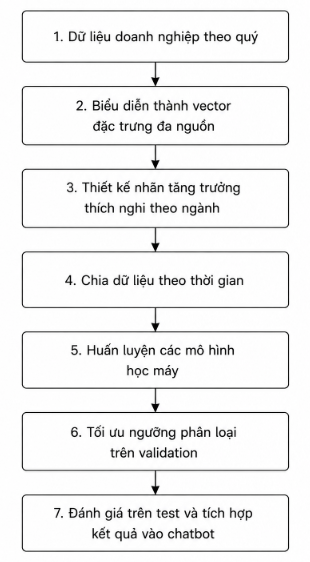
\includegraphics[width=0.9\textwidth,height=0.65\textheight,keepaspectratio]{figures/image2.png}
\caption{Quy trình tổng thể của phương pháp dự báo xu hướng tăng trưởng doanh nghiệp}
\label{fig:3-1}
\end{figure}

Ở tầng dữ liệu, hệ thống thu thập các nguồn thông tin liên quan đến doanh nghiệp, thị trường và bối cảnh kinh tế. Tầng đặc trưng đồng bộ dữ liệu về cùng đơn vị doanh nghiệp--quý và chuyển mỗi quan sát thành vector đầu vào. Tầng biến mục tiêu gán nhãn tăng trưởng mạnh dựa trên ngưỡng theo ngành cùng các điều kiện kiểm soát chất lượng tài chính. Trên tập dữ liệu đã gán nhãn, các mô hình Random Forest, XGBoost, LightGBM và Weighted Soft Voting được huấn luyện để ước lượng xác suất lớp dương. Kết quả cuối cùng được lưu để chatbot truy xuất và diễn giải bằng ngôn ngữ tự nhiên.

\begin{table}[H]
\centering
\caption{Vai trò các thành phần trong quy trình dự báo}
\label{tab:3-1}
\small
\setlength{\tabcolsep}{6pt}
\begin{tabular}{p{0.28\textwidth}p{0.62\textwidth}}
\toprule
\textbf{Thành phần} & \textbf{Vai trò} \\
\midrule
Tầng dữ liệu & Thu thập và đồng bộ dữ liệu tài chính, thị trường, kỹ thuật, vĩ mô, ngành và tin tức theo từng quý. \\
Tầng đặc trưng & Xây dựng các đặc trưng phản ánh tình hình tài chính, diễn biến giá, thanh khoản, chu kỳ và bối cảnh bên ngoài. \\
Tầng biến mục tiêu & Xác định nhãn tăng trưởng lợi nhuận mạnh bằng ngưỡng thích nghi theo ngành, kết hợp điều kiện ROA, ROE và lợi nhuận TTM. \\
Tầng mô hình & Huấn luyện các mô hình học máy, tối ưu ngưỡng phân loại và so sánh với các mô hình cơ sở. \\
Tầng ứng dụng & Truy xuất kết quả dự báo và diễn giải thông tin cho người dùng thông qua chatbot phân tích tài chính. \\
\bottomrule
\end{tabular}
\end{table}

\section{Tổ chức dữ liệu đầu vào và xây dựng đặc trưng}
Một quan sát trong tập dữ liệu tương ứng với doanh nghiệp \(i\) tại quý \(t\). Sau khi làm sạch, đồng bộ thời gian và tổng hợp đặc trưng, quan sát này được biểu diễn dưới dạng vector nhiều chiều:


\begin{equation}
x_{i,t}=[x^{fin}_{i,t},x^{market}_{i,t},x^{tech}_{i,t},x^{macro}_{t},x^{industry}_{i,t},x^{news}_{i,t}]
\end{equation}


Trong đó:
\begin{itemize}
  \item \(\boldsymbol{x}^{fin}_{i,t}\) gồm các biến tài chính như doanh thu, lợi nhuận, tài sản, vốn chủ sở hữu, nợ phải trả, dòng tiền hoạt động, ROA, ROE và các chỉ tiêu tăng trưởng.
  \item \(\boldsymbol{x}^{market}_{i,t}\) mô tả giao dịch của cổ phiếu, gồm giá, khối lượng, lợi suất, biến động và thanh khoản.
  \item \(\boldsymbol{x}^{tech}_{i,t}\) chứa các chỉ báo kỹ thuật được tạo từ dữ liệu giá và khối lượng, phản ánh xu hướng, động lượng và mức biến động.
  \item \(\boldsymbol{x}^{macro}_{t}\) biểu diễn điều kiện vĩ mô tại thời điểm quan sát, áp dụng chung cho thị trường thay vì riêng một doanh nghiệp.
  \item \(\boldsymbol{x}^{industry}_{i,t}\) mã hóa thông tin ngành để mô hình nhận biết khác biệt về mô hình kinh doanh và chu kỳ hoạt động.
  \item \(\boldsymbol{x}^{news}_{i,t}\) tổng hợp tín hiệu từ tin tức và sự kiện có liên quan đến doanh nghiệp hoặc ngành.
\end{itemize}

\begin{figure}[H]
\centering
\makebox[\textwidth][c]{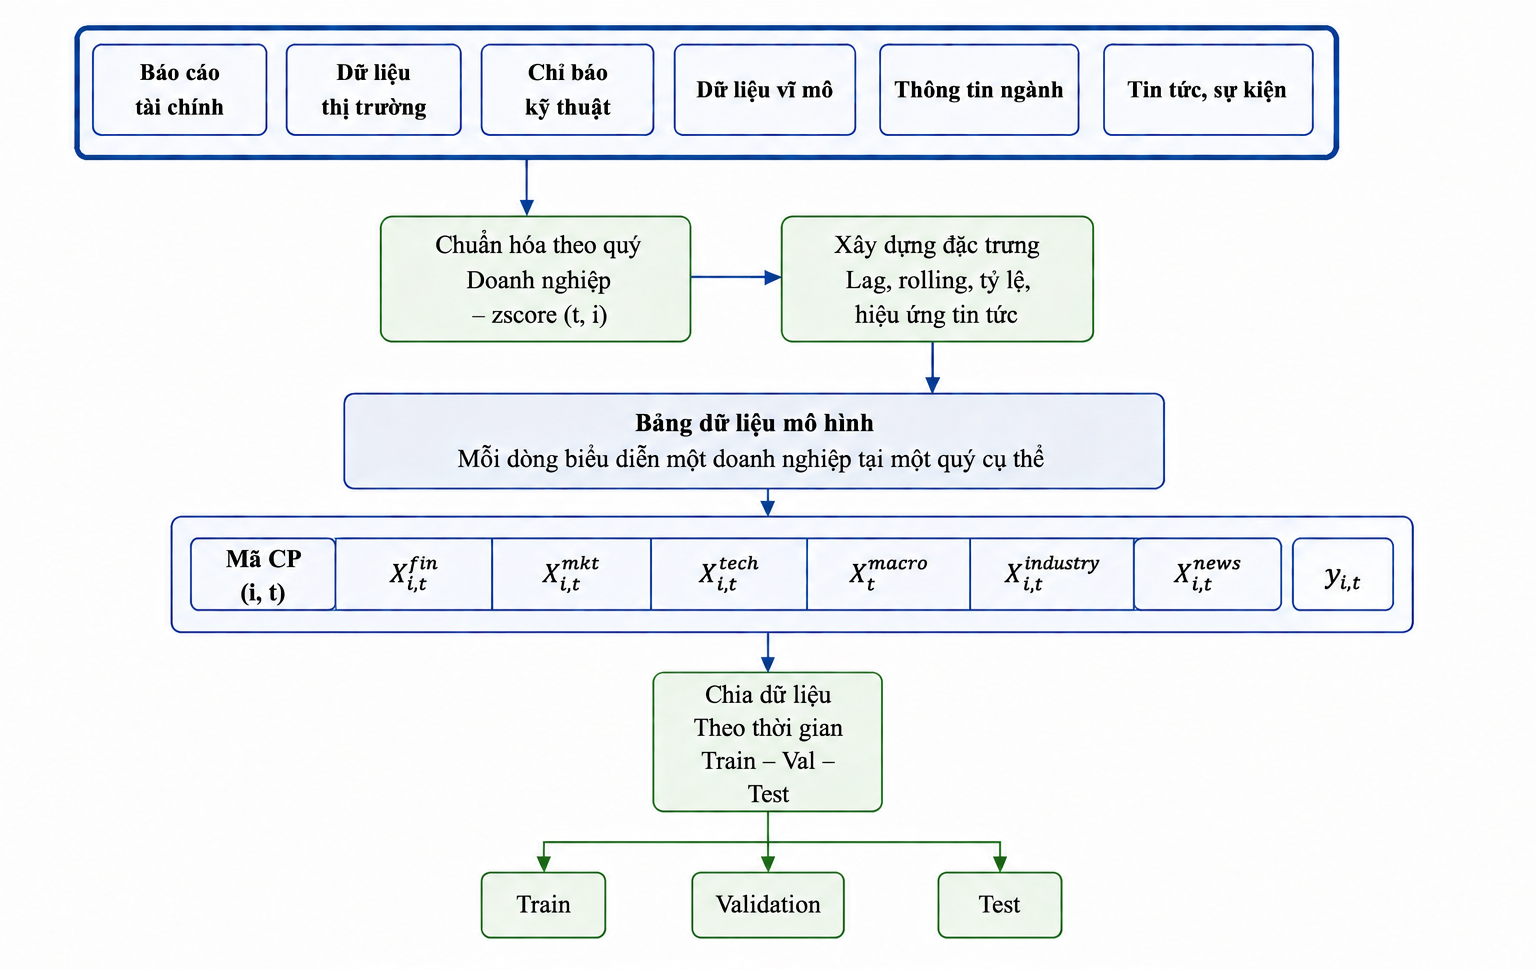
\includegraphics[width=1.15\textwidth]{figures/image10.png}}
\caption{Cấu trúc dữ liệu đầu vào và bảng dữ liệu mô hình}
\label{fig:data-structure}
\end{figure}

\subsection{Dữ liệu báo cáo tài chính}
Báo cáo tài chính cung cấp phần thông tin cốt lõi về hoạt động doanh nghiệp. Khóa luận sử dụng các khoản mục như doanh thu, lợi nhuận sau thuế, tổng tài sản, vốn chủ sở hữu, nợ phải trả, dòng tiền từ hoạt động kinh doanh, ROA, ROE và các biến tăng trưởng. Ngoài giá trị tại quý quan sát, hệ thống tạo thêm biến trễ và trung bình trượt để ghi nhận xu hướng tích lũy qua nhiều quý.

\subsection{Dữ liệu thị trường và chỉ báo kỹ thuật}
Dữ liệu thị trường cho biết cổ phiếu được giao dịch như thế nào qua thời gian, bao gồm giá, khối lượng, lợi suất, độ biến động và thanh khoản. Từ chuỗi giá và khối lượng, khóa luận xây dựng thêm RSI, MACD, khoảng cách so với đường trung bình động, stochastic và CCI. Những biến này bổ sung góc nhìn về kỳ vọng và phản ứng của nhà đầu tư đối với triển vọng doanh nghiệp.

\subsection{Dữ liệu vĩ mô và thông tin ngành}
Các biến vĩ mô như GDP, lạm phát, lãi suất, tỷ giá và tăng trưởng công nghiệp được đưa vào để mô tả điều kiện kinh tế chung. Mặc dù không gắn với riêng một doanh nghiệp, các biến này có thể ảnh hưởng đến chi phí vốn, nhu cầu thị trường và hiệu quả hoạt động của nhiều ngành. Thông tin ngành được sử dụng cho cả hai mục đích: hỗ trợ mô hình nhận diện đặc thù hoạt động và phục vụ bước xây dựng ngưỡng tăng trưởng thích nghi.

\subsection{Dữ liệu tin tức và sự kiện tài chính}
Tin tức và sự kiện tài chính được dùng như nguồn tín hiệu bổ sung cho dữ liệu định lượng. Các đặc trưng được tổng hợp gồm số lượng tin, điểm cảm xúc trung bình, số tin tích cực, số tin tiêu cực và nhóm sự kiện liên quan đến kết quả kinh doanh, ngành hoặc rủi ro doanh nghiệp. Để giữ đúng nguyên tắc thời gian, chỉ những thông tin đã xuất hiện tại hoặc trước quý quan sát mới được dùng làm đầu vào.

\section{Mô hình hóa bài toán dự báo}
Giả sử tập dữ liệu gồm \(N\) doanh nghiệp và \(T\) quý quan sát. Với doanh nghiệp \(i \in \{1,\ldots,N\}\) tại quý \(t \in \{1,\ldots,T\}\), hệ thống sử dụng vector \(x_{i,t}\in\mathbb{R}^{d}\) để dự báo trạng thái tăng trưởng lợi nhuận ở kỳ tương lai. Ký hiệu \(d\) là số đặc trưng còn lại sau các bước xử lý và chọn lọc.

Nhãn đầu ra của bài toán được ký hiệu là:


\begin{equation}
y_{i,t}\in\{0,1\}
\end{equation}


Trong đó, \(y_{i,t}=1\) biểu thị doanh nghiệp thuộc nhóm tăng trưởng lợi nhuận mạnh trong kỳ dự báo, còn \(y_{i,t}=0\) biểu thị doanh nghiệp không thuộc nhóm này. Mô hình cần học ánh xạ từ đặc trưng đầu vào sang xác suất lớp dương:


\begin{equation}
\hat p_{i,t}=P(y_{i,t}=1\mid x_{i,t};\theta)
\end{equation}


Trong đó, \(\theta\) là tập tham số của mô hình. Từ xác suất dự báo, nhãn dự báo cuối cùng được xác định thông qua ngưỡng phân loại \(\gamma\):


\begin{equation}
\hat y_{i,t}=
\begin{cases}
1, & \hat p_{i,t}\ge\gamma,\\
0, & \hat p_{i,t}<\gamma.
\end{cases}
\end{equation}


Điểm cần kiểm soát là thời điểm hình thành dữ liệu. Vector \(x_{i,t}\) chỉ chứa thông tin biết được đến quý \(t\), trong khi nhãn \(y_{i,t}\) được xác định từ kết quả sau thời điểm đó. Vì vậy, nhãn tương lai không được tham gia vào bất kỳ bước xây dựng đặc trưng nào.

\section{Xây dựng biến mục tiêu thích nghi theo ngành}
Biến mục tiêu quyết định trực tiếp mô hình sẽ học tín hiệu nào từ dữ liệu. Nếu dùng một ngưỡng tăng trưởng chung cho toàn bộ thị trường, những ngành có lợi nhuận biến động mạnh có thể tạo ra nhiều nhãn dương hơn, trong khi doanh nghiệp nổi bật ở ngành ổn định lại dễ bị bỏ qua. Để giảm thiên lệch này, khóa luận xây dựng nhãn dựa trên ngưỡng riêng theo ngành.

Gọi \(g_{i,t}\) là mức tăng trưởng lợi nhuận của doanh nghiệp \(i\) trong kỳ dự báo:


\begin{equation}
g_{i,t}=\frac{\mathrm{NP}_{i,t+h}-\mathrm{NP}_{i,t}}{|\mathrm{NP}_{i,t}|+\epsilon}\times 100
\end{equation}


Trong đó, \(\mathrm{NP}_{i,t}\) là lợi nhuận được sử dụng làm cơ sở xây dựng biến mục tiêu tại quý \(t\), \(h\) là kỳ hạn dự báo và \(\epsilon\) là hằng số rất nhỏ để tránh chia cho 0. Với mỗi ngành \(c\), ngưỡng tăng trưởng mạnh được xác định bằng phân vị \(s\) của tăng trưởng lợi nhuận trong tập huấn luyện:


\begin{equation}
\tau^{growth}_{c}=Q_s(g_{i,t}\mid industry_i=c)
\end{equation}


Trong đó, \(Q_s\) là phân vị được chọn và \(industry_i=c\) biểu thị doanh nghiệp \(i\) thuộc ngành \(c\). Toàn bộ ngưỡng được học từ tập huấn luyện, sau đó giữ cố định khi áp dụng cho tập xác thực và tập kiểm thử để không đưa thông tin tương lai vào quá trình gán nhãn.

Bên cạnh điều kiện tăng trưởng, khóa luận bổ sung bộ lọc chất lượng tài chính. Mục đích là tránh gán nhãn dương cho các trường hợp tăng trưởng cao chủ yếu do nền lợi nhuận quá thấp hoặc do biến động bất thường. Cụ thể, doanh nghiệp cần có ROA hoặc ROE không quá thấp so với mặt bằng ngành:


\begin{equation}
\mathrm{ROA}_{i,t}\ge\tau^{ROA}_{c}\quad \text{hoặc}\quad \mathrm{ROE}_{i,t}\ge\tau^{ROE}_{c}
\end{equation}


Ngoài ra, lợi nhuận lũy kế bốn quý gần nhất cũng được sử dụng để kiểm tra nền lợi nhuận:


\begin{equation}
\mathrm{NetProfitTTM}_{i,t}\ge\tau^{profit}_{c}
\end{equation}


Trong đó, \(\tau^{ROA}_{c}\), \(\tau^{ROE}_{c}\) và \(\tau^{profit}_{c}\) là các ngưỡng chất lượng tài chính được tính theo từng ngành trên tập huấn luyện.

Nhãn mục tiêu được xác định như sau:


\begin{equation}
y_{i,t}=
\begin{cases}
1, & \text{nếu } g_{i,t}>\tau^{growth}_{c}\text{ và thỏa điều kiện chất lượng tài chính},\\
0, & \text{nếu } g_{i,t}\le0,\\
\text{Loại bỏ}, & \text{các trường hợp trung gian.}
\end{cases}
\end{equation}


Những quan sát nằm giữa hai cực, tức có tăng trưởng dương nhưng chưa đủ mạnh hoặc không đạt điều kiện chất lượng tài chính, được loại khỏi tập huấn luyện. Việc này làm giảm số mẫu mơ hồ và giúp mô hình tập trung vào ranh giới rõ hơn giữa nhóm tăng trưởng mạnh và nhóm không tăng trưởng.

\begin{center}
\begin{minipage}{\textwidth}
\hrule
\vspace{2pt}
{{\textbf{Thuật toán 3.1 Xây dựng nhãn tăng trưởng thích nghi theo ngành}}}
\hrule
\vspace{2pt}
\noindent\textbf{Đầu vào:} Dữ liệu theo quý \(D\), mã doanh nghiệp \(i\), thời điểm \(t\), ngành \(c\), lợi nhuận thuộc cổ đông công ty mẹ \(NP\), ROA, ROE, lợi nhuận TTM, kỳ hạn dự báo \(h\), phân vị \(Q_s,Q_q\), số mẫu tối thiểu \(n_{\min}\).

\noindent\textbf{Đầu ra:} Tập dữ liệu đã gán nhãn \(D^*\), nhãn mục tiêu \(y_{i,t}\), bộ ngưỡng ngành \(\Theta\).

\vspace{2pt}
\setlength{\tabcolsep}{2pt}
\renewcommand{\arraystretch}{1.05}
\begin{tabular}{@{}r p{0.52\linewidth}@{\hspace{0.1\linewidth}}p{0.30\linewidth}@{}}
1: & \(D_{tr},D_{val},D_{te}\leftarrow \mathrm{TimeSplit}(D)\) & \(\triangleright\) Chia theo thời gian\\
2: & \(\Theta\leftarrow\varnothing,\quad D^*\leftarrow\varnothing,\quad \Theta_0\leftarrow \mathrm{Quantile}(D_{tr})\) & \(\triangleright\) Khởi tạo và ngưỡng toàn cục\\
3: & \textbf{for all} ngành \(c\in D_{tr}\) \textbf{do} & \\
4: & \quad \(G_c\leftarrow\{g_{i,t}: industry_i=c,(i,t)\in D_{tr}\}\) & \(\triangleright\) Tập tăng trưởng ngành\\
5: & \quad \textbf{if} \(|G_c|\ge n_{\min}\) \textbf{then} \(\Theta_c\leftarrow\mathrm{Quantile}_c(G_c,ROA,ROE,NP^{TTM})\) & \(\triangleright\) Ngưỡng theo ngành\\
6: & \quad \textbf{else} \(\Theta_c\leftarrow\Theta_0\) & \(\triangleright\) Ngưỡng toàn cục\\
7: & \quad \(\tau^{growth}_{c}\leftarrow\max(0,\tau^{growth}_{c}),\quad \tau^{profit}_{c}\leftarrow\max(0,\tau^{profit}_{c})\) & \(\triangleright\) Chặn ngưỡng âm\\
8: & \quad \(\Theta\leftarrow\Theta\cup\Theta_c\) & \(\triangleright\) Lưu ngưỡng\\
9: & \textbf{end for} & \\
10: & \textbf{for all} \((i,t)\in D_{tr}\cup D_{val}\cup D_{te}\) \textbf{do} & \\
11: & \quad \(c\leftarrow industry_i,\quad g_{i,t}\leftarrow (NP_{i,t+h}-NP_{i,t})/(|NP_{i,t}|+\epsilon)\times100\) & \(\triangleright\) Tăng trưởng tương lai\\
12: & \quad \(q_{i,t}\leftarrow[(ROA_{i,t}\ge\tau^{ROA}_{c})\vee(ROE_{i,t}\ge\tau^{ROE}_{c})]\wedge[NP^{TTM}_{i,t}\ge\tau^{profit}_{c}]\) & \(\triangleright\) Kiểm tra chất lượng\\
13: & \quad \textbf{if} \((g_{i,t}>\tau^{growth}_{c})\wedge q_{i,t}\) \textbf{then} \(y_{i,t}\leftarrow1\) & \(\triangleright\) Tăng trưởng mạnh\\
14: & \quad \textbf{else if} \(g_{i,t}\le0\) \textbf{then} \(y_{i,t}\leftarrow0\) & \(\triangleright\) Không tăng trưởng\\
15: & \quad \textbf{else} \(y_{i,t}\leftarrow\text{Loại bỏ}\) & \(\triangleright\) Mẫu trung gian\\
16: & \quad \textbf{if} \(y_{i,t}\ne\text{Loại bỏ}\) \textbf{then} \(D^*\leftarrow D^*\cup\{(x_{i,t},y_{i,t})\}\) & \(\triangleright\) Giữ mẫu hợp lệ\\
17: & \textbf{end for} & \\
18: & \textbf{return} \(D^*,y,\Theta\) & \\
\end{tabular}
\vspace{2pt}
\hrule
\end{minipage}
\end{center}

Thuật toán trên có ba điểm cần lưu ý. Thứ nhất, dữ liệu được chia theo thời gian thành \(D_{train}\), \(D_{val}\) và \(D_{test}\); chỉ \(D_{train}\) được dùng để tính ngưỡng. Thứ hai, bộ \(\Theta\) lưu các ngưỡng riêng của từng ngành, gồm ngưỡng tăng trưởng và các ngưỡng chất lượng tài chính. Thứ ba, biến \(quality\) đóng vai trò kiểm tra nền tảng tài chính để hạn chế những nhãn dương phát sinh từ nền lợi nhuận thấp.

Sau khi thuật toán chạy xong, mỗi quan sát được đưa vào một trong ba trạng thái: tăng trưởng mạnh, không tăng trưởng hoặc loại bỏ. Chỉ các quan sát còn lại trong \(D^*\) được sử dụng ở bước huấn luyện mô hình phân loại.

Ví dụ, mức tăng trưởng lợi nhuận 30\% có thể là tín hiệu nổi bật trong một ngành có lợi nhuận ổn định như ngân hàng. Tuy nhiên, cùng mức tăng trưởng đó có thể chưa đủ đặc biệt ở một ngành có chu kỳ lợi nhuận dao động mạnh hơn. Do đó, so sánh doanh nghiệp với chính mặt bằng ngành giúp nhãn mục tiêu sát thực tế hơn.

\section{Huấn luyện mô hình và tối ưu ngưỡng phân loại}
Sau khi hoàn tất tập đặc trưng và nhãn mục tiêu, các mô hình được huấn luyện để ước lượng xác suất doanh nghiệp thuộc lớp tăng trưởng lợi nhuận mạnh. Với mô hình \(m\), xác suất dự báo được ký hiệu là:


\begin{equation}
\hat p^{(m)}_{i,t}=f_m(x_{i,t};\theta_m)
\end{equation}


Trong đó, \(f_m\) là hàm dự báo của mô hình thứ \(m\), còn \(\theta_m\) là tập tham số tương ứng. Random Forest, XGBoost và LightGBM được dùng làm các mô hình phân loại chính vì chúng phù hợp với dữ liệu bảng và có khả năng học quan hệ phi tuyến giữa nhiều nhóm đặc trưng.

Ridge Regression và ARIMA được sử dụng như các mô hình cơ sở để đối chiếu. Ridge Regression dự báo giá trị tăng trưởng liên tục rồi chuyển sang nhãn phân loại, trong khi ARIMA khai thác cấu trúc thời gian của chuỗi lịch sử. Việc đưa hai mô hình này vào thực nghiệm giúp đánh giá liệu mô hình học máy đa biến có cải thiện kết quả so với cách tiếp cận đơn giản hơn hay không.

Để tăng tính ổn định, khóa luận áp dụng Weighted Soft Voting. Xác suất cuối cùng là trung bình có trọng số của xác suất dự báo từ các mô hình con:


\begin{equation}
\hat p_{i,t}=\frac{\sum_{m=1}^{M}w_m\hat p^{(m)}_{i,t}}{\sum_{m=1}^{M}w_m}
\end{equation}


Trong đó, \(M\) là số mô hình được kết hợp, \(w_m\) là trọng số của mô hình thứ \(m\), và \(\hat p^{(m)}_{i,t}\) là xác suất dự báo của mô hình thứ \(m\). Trọng số được xác định dựa trên hiệu quả của mô hình trên tập xác thực.

Vì mô hình trả về xác suất, cần một ngưỡng \(\gamma\) để chuyển xác suất thành nhãn. Ngưỡng 0.5 không luôn phù hợp, nhất là khi hai lớp không cân bằng hoặc khi mục tiêu đánh giá ưu tiên F1-score hay Balanced Accuracy. Do đó, \(\gamma\) được lựa chọn trên tập xác thực thay vì cố định trước.

\begin{figure}[H]
\centering
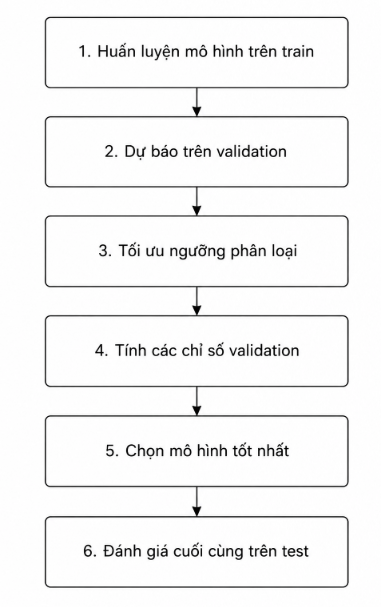
\includegraphics[width=0.9\textwidth,height=0.65\textheight,keepaspectratio]{figures/image3.png}
\caption{Quy trình lựa chọn mô hình và tối ưu ngưỡng phân loại}
\label{fig:3-2}
\end{figure}

Quy trình lựa chọn mô hình tuân theo thứ tự thời gian. Tập huấn luyện dùng để học tham số và tính ngưỡng mục tiêu; tập xác thực dùng để chọn mô hình, xác định trọng số voting và tối ưu ngưỡng phân loại; tập kiểm thử chỉ được dùng ở bước cuối để đánh giá khả năng tổng quát hóa.

\section{Tích hợp kết quả dự báo vào chatbot phân tích tài chính}
Ngoài phần mô hình dự báo, khóa luận xây dựng thêm lớp chatbot để người dùng tra cứu kết quả thuận tiện hơn. Chatbot không tham gia huấn luyện mô hình; nó hoạt động như lớp ứng dụng phía trên, nhận câu hỏi, truy xuất kết quả và trình bày lại thông tin theo ngôn ngữ tự nhiên.

\begin{figure}[H]
\centering
\resizebox{\textwidth}{!}{%
\begin{tikzpicture}[
  font=\small,
  node distance=0.85cm and 0.95cm,
  arrow/.style={-{Latex[length=2.2mm]}, line width=0.65pt, draw=thesisblue},
  queryarrow/.style={{Latex[length=2.0mm]}-{Latex[length=2.0mm]}, line width=0.65pt, draw=thesisblue},
  block/.style={draw=thesisboxline, fill=white, rounded corners=1.5mm, align=center,
    minimum height=1.0cm, text width=3.25cm, inner sep=6pt},
  process/.style={block, fill=blue!4},
  store/.style={block, fill=gray!7},
  model/.style={block, fill=green!7},
  userbox/.style={block, fill=orange!9}
]

\node[userbox] (user)
  {Người dùng\\\footnotesize Câu hỏi phân tích};
\node[process, right=0.85cm of user] (nlu)
  {Nhận diện truy vấn\\\footnotesize Mã, quý, ý định};
\node[process, right=0.85cm of nlu] (retrieve)
  {Truy xuất thông tin\\\footnotesize Dự báo và đặc trưng};
\node[process, right=0.85cm of retrieve] (generate)
  {Tổng hợp diễn giải\\\footnotesize Tạo câu trả lời};
\node[userbox, right=0.85cm of generate] (answer)
  {Phản hồi\\\footnotesize câu trả lời, lý do};

\node[store, below=1.55cm of retrieve, xshift=-2.65cm] (predstore)
  {Kết quả\\\footnotesize Xác suất, nhãn};
\node[store, below=1.55cm of retrieve, xshift=2.65cm] (featurestore)
  {Đặc trưng\\\footnotesize Tài chính, ngành, tin tức};
\node[model, below=1.75cm of predstore] (models)
  {Mô hình dự báo\\\footnotesize};
\node[store, below=0.95cm of featurestore] (processed)
  {Dữ liệu đã xử lý\\\footnotesize Đa nguồn theo quý};

\draw[arrow] (user) -- (nlu);
\draw[arrow] (nlu) -- (retrieve);
\draw[arrow] (retrieve) -- (generate);
\draw[arrow] (generate) -- (answer);
\draw[arrow] (retrieve.south) -- ++(0,-0.45) -| (featurestore.north);
\draw[arrow] (featurestore) -- (processed);
\draw[arrow] (processed) -- (models);
\draw[arrow] (models) -- (predstore);
\draw[arrow] (predstore.north) -- ++(0,0.55) -| (generate.south);

\node[draw=thesisboxline, rounded corners=2mm, fit=(nlu)(retrieve)(generate),
  inner xsep=0.22cm, inner ysep=0.28cm, label={[font=\bfseries\footnotesize, text=thesisblue]above:Lớp chatbot}] {};
\node[draw=thesisboxline, rounded corners=2mm, fit=(predstore)(featurestore)(models)(processed),
  inner xsep=0.25cm, inner ysep=0.3cm, label={[font=\bfseries\footnotesize, text=thesisblue]below:Tầng dữ liệu và mô hình dự báo}] {};

\end{tikzpicture}%
}
\caption{Mô tả kiến trúc tích hợp mô hình dự báo vào hệ thống chatbot phân tích tài chính}
\label{fig:3-3}
\end{figure}

Khi nhận câu hỏi về một mã cổ phiếu, chatbot trước hết xác định mã, thời gian, ngành hoặc ý định truy vấn. Sau đó, hệ thống lấy các thông tin liên quan từ dữ liệu đã xử lý, gồm nhãn dự báo, xác suất tăng trưởng mạnh, một số đặc trưng tài chính quan trọng và thông tin ngành. Các dữ liệu này được tổng hợp thành câu trả lời ngắn gọn để người dùng có thể hiểu kết quả mô hình mà không cần mở trực tiếp các bảng dự báo.

Vai trò của chatbot vì vậy là rút ngắn khoảng cách giữa kết quả mô hình và người dùng cuối. Các phản hồi chỉ có ý nghĩa tham khảo, hỗ trợ phân tích và không được thiết kế để đưa ra quyết định mua bán cổ phiếu thay cho người dùng.

\chapter{Thực nghiệm và đánh giá kết quả}
Chương này mô tả phần kiểm thử hệ thống trên dữ liệu doanh nghiệp niêm yết tại Việt Nam. Thay vì chỉ báo cáo một mô hình tốt nhất, phần thực nghiệm đối chiếu nhiều thuật toán trên cùng dữ liệu theo quý để xem mô hình nào nhận diện nhóm tăng trưởng mạnh ổn định hơn.

\section{Dữ liệu thực nghiệm}
Dữ liệu thực nghiệm gồm các doanh nghiệp niêm yết được sắp xếp theo từng quý. Một dòng dữ liệu biểu diễn một mã cổ phiếu tại một thời điểm quan sát, còn các cột là đặc trưng được tạo từ nhiều nguồn. Cách tổ chức này phù hợp với bài toán dự báo vì mọi thông tin đầu vào đều phải tồn tại trước kỳ cần dự báo.

Giai đoạn chính được lấy từ 2018Q1 đến 2026Q1. Mốc 2018Q1 được chọn vì dữ liệu lợi nhuận theo quý từ giai đoạn này đầy đủ hơn cho việc tạo nhãn. Dữ liệu thị trường có thể kéo dài hơn, nhưng nếu thiếu lợi nhuận theo quý thì không thể xác định biến mục tiêu của khóa luận.

\begin{longtable}{|p{0.46\textwidth}|p{0.46\textwidth}|}
\caption{Thống kê tổng quan bộ dữ liệu thực nghiệm}\label{tab:4-1}\\
\hline
\textbf{Thành phần} & \textbf{Giá trị} \\
\hline
Số mã cổ phiếu & 96 \\
\hline
Giai đoạn dữ liệu & 2018Q1 – 2026Q1 \\
\hline
Số dòng dữ liệu & 3108 \\
\hline
Số đặc trưng sau xử lý & Khoảng 466 \\
\hline
Số nhóm ngành cấp 1 & 9 \\
\hline
Số nhóm ngành cấp 2 & 15 \\
\hline
Đơn vị quan sát & Doanh nghiệp - quý \\
\hline
\end{longtable}
Bộ đặc trưng có hai nhóm lớn: thông tin nội tại doanh nghiệp và thông tin bên ngoài. Nhóm nội tại gồm doanh thu, lợi nhuận, tài sản, vốn chủ sở hữu, nợ phải trả, dòng tiền hoạt động, ROA và ROE. Nhóm thị trường gồm giá, khối lượng, lợi suất theo quý, độ biến động và thanh khoản; từ đó tạo thêm RSI, MACD, khoảng cách đến đường trung bình động, stochastic và CCI.

Ở cấp bối cảnh, tập dữ liệu bổ sung GDP, lạm phát, lãi suất, tỷ giá và tăng trưởng công nghiệp. Ngành được dùng để phân nhóm doanh nghiệp và tính ngưỡng nhãn riêng. Tin tức/sự kiện không được đưa vào dưới dạng văn bản thô mà được tổng hợp thành số lượng tin, điểm cảm xúc, số tin tích cực/tiêu cực và nhóm sự kiện liên quan.

Thực nghiệm sử dụng biến \textit{target\_\allowbreak adaptive\_\allowbreak strong\_\allowbreak profit\_\allowbreak up\_\allowbreak 1q}. Nhãn bằng 1 khi doanh nghiệp thuộc nhóm tăng trưởng lợi nhuận mạnh ở quý tiếp theo theo chuẩn ngành; nhãn bằng 0 khi doanh nghiệp không đạt điều kiện đó. Cách tạo nhãn này giúp hạn chế việc so sánh trực tiếp các ngành có biên độ lợi nhuận rất khác nhau.

Hai cấu hình nhãn thích nghi theo ngành được dùng để so sánh được liệt kê trong \textit{Bảng 4.2}.

\begin{table}[H]
\centering
\caption{Các cấu hình biến mục tiêu thích nghi theo ngành được sử dụng}
\label{tab:4-2}
\small
\setlength{\tabcolsep}{3pt}
\begin{tabular}{|L{0.18\textwidth}|L{0.24\textwidth}|L{0.22\textwidth}|L{0.22\textwidth}|}
\hline
\textbf{Cấu hình} & \textbf{Ngưỡng tăng trưởng mạnh} & \textbf{Ngưỡng ROA/ROE thấp} & \textbf{Ngưỡng net profit TTM thấp} \\
\hline
\textit{s70\_q20\_p20} & Percentile 70\% theo ngành & Percentile 20\% theo ngành & Percentile 20\% theo ngành \\
\hline
\textit{s80\_q10\_p10} & Percentile 80\% theo ngành & Percentile 10\% theo ngành & Percentile 10\% theo ngành \\
\hline
\end{tabular}
\end{table}
\section{Thiết lập môi trường và tham số thực nghiệm}
Môi trường chạy thực nghiệm được trình bày trong \textit{Bảng 4.3}. Các thông tin này được ghi lại để đảm bảo kết quả có thể được kiểm tra lại trong cùng điều kiện triển khai.

\begin{table}[H]
\centering
\caption{Cấu hình phần cứng và môi trường phần mềm}
\label{tab:4-3}
\small
\setlength{\tabcolsep}{6pt}
\begin{tabular}{p{0.28\textwidth}p{0.62\textwidth}}
\toprule
\textbf{Thành phần} & \textbf{Chi tiết kỹ thuật} \\
\midrule
\multicolumn{2}{l}{\textbf{Phần cứng}} \\
CPU & AMD Ryzen 5 5600H with Radeon Graphics (12 CPUs), \textasciitilde{}3.3GHz \\
GPU & AMD Radeon Graphics \\
RAM & 16 GB RAM \\
\addlinespace
\multicolumn{2}{l}{\textbf{Phần mềm}} \\
OS & Windows 11 Home Single Language 64-bit \\
Ngôn ngữ & Python 3.10 \\
IDE & Visual Studio Code \\
Thư viện chính & pandas, numpy, scikit-learn, xgboost, lightgbm, statsmodels, matplotlib, joblib \\
\bottomrule
\end{tabular}
\end{table}
Các thử nghiệm được chạy bằng Python. pandas và numpy xử lý bảng dữ liệu; scikit-learn đảm nhiệm pipeline huấn luyện và đánh giá; xgboost, lightgbm và statsmodels cung cấp các mô hình chính; matplotlib dùng để trực quan hóa; joblib hỗ trợ lưu đối tượng mô hình.

Dữ liệu không được chia ngẫu nhiên mà được tách theo thời gian. Tập train dùng cho việc học tham số và tính ngưỡng theo ngành. Tập validation dùng để chọn threshold, chọn mô hình và tính trọng số voting. Tập test được giữ đến cuối để đo kết quả ngoài mẫu.

Các mô hình kiểm thử gồm Random Forest, ExtraTrees, GradientBoosting, HistGradientBoosting, XGBoost, LightGBM và Weighted Soft Voting. Ridge Regression và ARIMA được dùng làm baseline để so sánh với nhóm mô hình khai thác nhiều đặc trưng.

\textit{Bảng 4.4} ghi lại các tham số chính. Phần thực nghiệm ưu tiên kiểm tra ảnh hưởng của thiết kế target và sự khác biệt giữa các mô hình, thay vì tìm kiếm siêu tham số sâu cho từng thuật toán.

\begin{table}[H]
\centering
\caption{Tham số cấu hình thực nghiệm chính}
\label{tab:4-4}
\small
\setlength{\tabcolsep}{5pt}
\begin{tabular}{p{0.24\textwidth}p{0.34\textwidth}p{0.30\textwidth}}
\toprule
\textbf{Hạng mục} & \textbf{Tham số} & \textbf{Giá trị} \\
\midrule
Target & Biến mục tiêu chính & \textit{target\_\allowbreak adaptive\_\allowbreak strong\_\allowbreak profit\_\allowbreak up} \\
Adaptive group & Nhóm tính ngưỡng & Ngành cấp 1 \\
\addlinespace
Cấu hình target chính & Strong quantile & 0.8 \\
 & ROA/ROE quality quantile & 0.1 \\
 & Profit TTM quantile & 0.1 \\
\addlinespace
Cấu hình so sánh & Strong quantile & 0.7 \\
 & ROA/ROE quality quantile & 0.2 \\
 & Profit TTM quantile & 0.2 \\
\addlinespace
Lựa chọn mô hình & Selection metric & Validation F1-score \\
Tối ưu ngưỡng & Threshold metric & F1-score \\
Voting & Voting weight metric & Validation Balanced Accuracy \\
\addlinespace
Feature filtering & Min feature non-null & 0.15 \\
Feature filtering & Max feature correlation & 0.98 \\
\bottomrule
\end{tabular}
\end{table}
Đầu ra của mô hình phân loại là xác suất lớp dương. Threshold được chọn trên validation thay vì cố định ở 0.5, vì bài toán cần cân bằng giữa việc phát hiện đúng nhóm tăng trưởng mạnh và việc tránh dự báo dương sai.

Với Weighted Soft Voting, xác suất lớp dương từ các mô hình con được tổng hợp bằng trung bình có trọng số. Trọng số được xác định dựa trên kết quả validation, giúp mô hình kết hợp ưu tiên các mô hình con có hiệu quả tốt hơn thay vì xem mọi dự báo là ngang nhau.

\section{Kết quả thực nghiệm và phân tích}
Sau khi chuẩn bị dữ liệu và cấu hình mô hình, kết quả được tổng hợp trên tập test. Phần phân tích tập trung vào hai câu hỏi: cấu hình target nào phù hợp hơn và mô hình nào cho tín hiệu dự báo đáng tin cậy hơn.

\subsection{Kết quả so sánh các mô hình}
{\scriptsize
\setlength{\tabcolsep}{2pt}
\begin{longtable}{|L{0.12\textwidth}|L{0.17\textwidth}|C{0.09\textwidth}|C{0.12\textwidth}|C{0.09\textwidth}|C{0.09\textwidth}|C{0.08\textwidth}|C{0.07\textwidth}|}
\caption{Kết quả thực nghiệm trên tập kiểm thử đối với hai cấu hình biến mục tiêu thích nghi theo ngành s70\_q20\_p20 và s80\_q10\_p10.}\label{tab:4-5}\\
\hline
\textbf{Cấu hình} & \textbf{Mô hình} & \textbf{Accuracy} & \textbf{Balanced Accuracy} & \textbf{Precision} & \textbf{Recall} & \textbf{F1-score} & \textbf{AUC} \\
\hline
s80\_q10\_p10 & LightGBM & 0.800 & 0.783 & 0.602 & 0.747 & 0.667 & 0.848 \\
\hline
s80\_q10\_p10 & Weighted Soft Voting & 0.825 & 0.775 & 0.676 & 0.667 & 0.671 & 0.860 \\
\hline
s80\_q10\_p10 & XGBoost & 0.818 & 0.775 & 0.654 & 0.680 & 0.667 & 0.860 \\
\hline
s80\_q10\_p10 & Random Forest & 0.814 & 0.755 & 0.662 & 0.627 & 0.644 & 0.860 \\
\hline
s80\_q10\_p10 & ARIMA & 0.582 & 0.558 & 0.322 & 0.507 & 0.394 & - \\
\hline
s70\_q20\_p20 & LightGBM & 0.771 & 0.745 & 0.673 & 0.661 & 0.667 & 0.797 \\
\hline
s70\_q20\_p20 & ExtraTrees & 0.748 & 0.743 & 0.617 & 0.725 & 0.667 & 0.800 \\
\hline
s70\_q20\_p20 & Weighted Soft Voting & 0.761 & 0.718 & 0.685 & 0.578 & 0.627 & 0.812 \\
\hline
s70\_q20\_p20 & Random Forest & 0.755 & 0.705 & 0.686 & 0.541 & 0.605 & 0.793 \\
\hline
s70\_q20\_p20 & ARIMA & 0.475 & 0.540 & 0.373 & 0.752 & 0.498 & - \\
\hline
s70\_q20\_p20 & Ridge & 0.446 & 0.561 & 0.379 & 0.936 & 0.540 & 0.555 \\
\hline
\end{longtable}
}
\begin{figure}[htbp]
\centering
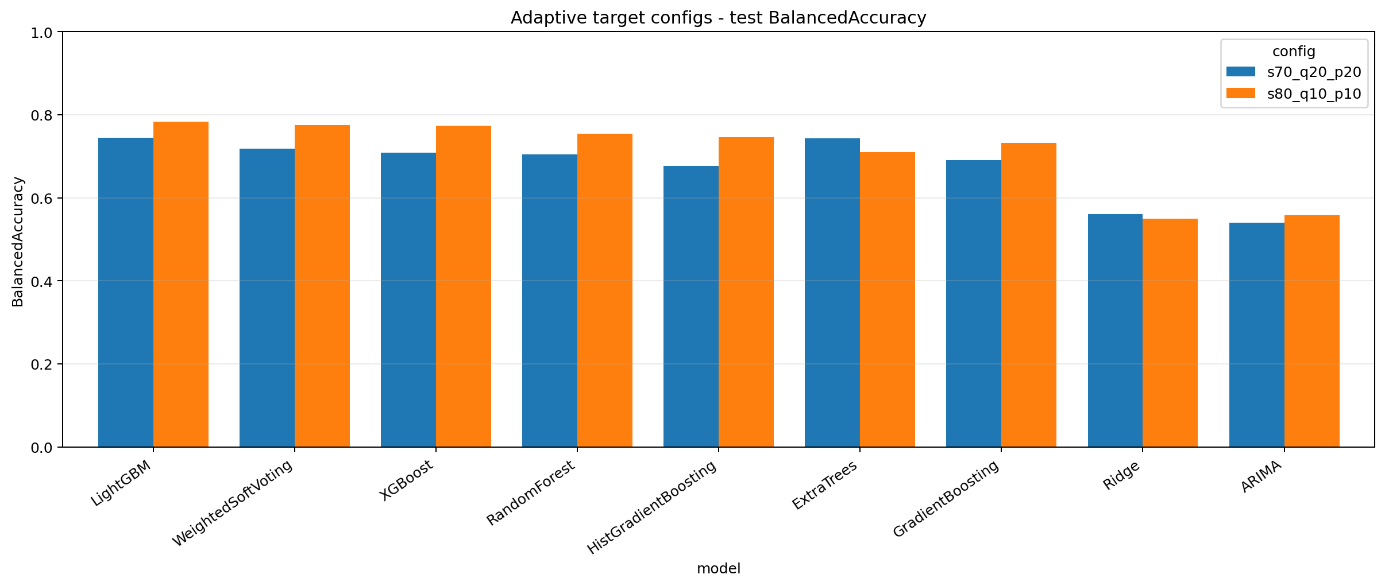
\includegraphics[width=0.9\textwidth]{figures/image5.png}
\caption{So sánh Balanced Accuracy của các mô hình}
\label{fig:4-1}
\end{figure}

\textit{Bảng 4.5} cho thấy \textit{s80\_q10\_p10} là cấu hình tốt hơn trong hầu hết chỉ số chính. LightGBM đạt Balanced Accuracy 0.783, cao nhất trong bảng. Weighted Soft Voting đạt Accuracy 0.825 và F1-score 0.671. Theo AUC, Weighted Soft Voting, XGBoost và Random Forest cùng đạt 0.860. Các kết quả này ủng hộ việc dùng mô hình cây và ensemble cho dữ liệu bảng tài chính.

\subsection{Phân tích cấu hình biến mục tiêu thích nghi theo ngành}
\begin{figure}[H]
\centering
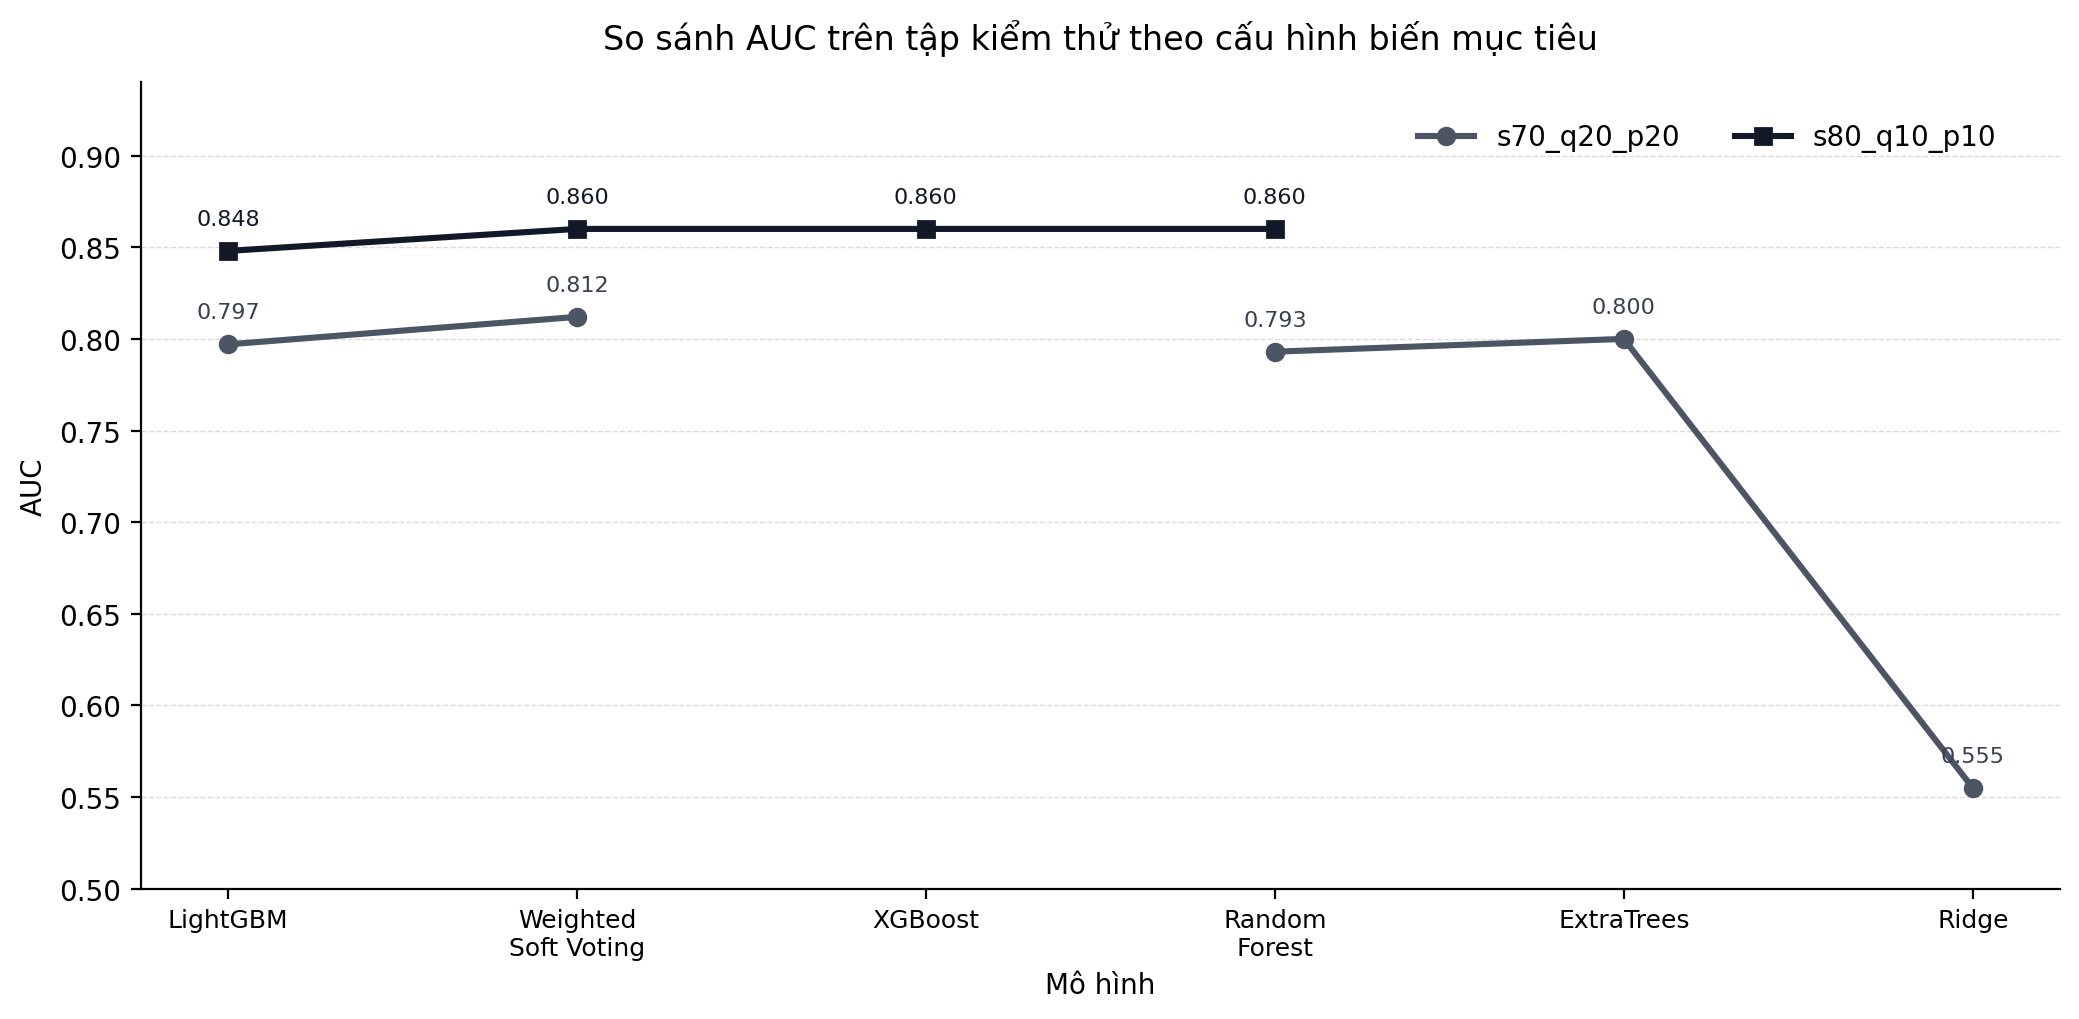
\includegraphics[width=0.9\textwidth]{figures/auc_comparison_test.png}
\caption{So sánh AUC giữa hai cấu hình biến mục tiêu thích nghi theo ngành}
\label{fig:4-3}
\end{figure}

Hai cấu hình trong thực nghiệm khác nhau ở độ chặt khi gán nhãn dương. Cấu hình \textit{s70\_q20\_p20} dùng phân vị 70\% của tăng trưởng theo ngành, còn \textit{s80\_q10\_p10} nâng ngưỡng tăng trưởng lên phân vị 80\%. Vì vậy, \textit{s80\_q10\_p10} chỉ giữ lại những quan sát nổi bật hơn trong từng ngành.

Khi ngưỡng tăng trưởng được đặt chặt hơn, lớp dương gồm các trường hợp rõ ràng hơn. Vì vậy, dù số mẫu dương giảm, mô hình vẫn học được ranh giới tốt hơn và đạt AUC, Balanced Accuracy cao hơn.

Ngược lại, \textit{s70\_q20\_p20} mở rộng lớp dương nên có thể đưa vào nhiều trường hợp chỉ tăng trưởng ở mức trung bình. Các mẫu này làm nhiệm vụ phân loại khó hơn vì chúng nằm gần ranh giới giữa hai lớp. Từ kết quả thực nghiệm, \textit{s80\_q10\_p10} được xem là cấu hình target phù hợp hơn cho các phân tích chính.

\subsection{Phân tích các mô hình tốt nhất}
Trong các mô hình đã thử nghiệm, bốn mô hình đáng chú ý nhất là LightGBM, Weighted Soft Voting, XGBoost và Random Forest.

LightGBM có Balanced Accuracy cao nhất và đồng thời đạt Recall tốt. Kết quả này cho thấy mô hình thiên về việc phát hiện được nhiều doanh nghiệp tăng trưởng mạnh thực tế hơn, dù điều đó có thể làm số dự báo dương sai tăng lên.

Weighted Soft Voting nổi bật ở F1-score và AUC. Việc tổng hợp xác suất từ nhiều mô hình con giúp kết quả bớt phụ thuộc vào một thuật toán riêng lẻ, đồng thời cân bằng tốt hơn giữa khả năng phát hiện lớp dương và mức độ chính xác của dự báo dương.

XGBoost đạt kết quả rất gần với Weighted Soft Voting, đặc biệt ở AUC 0.860. Điều này phù hợp với đặc điểm của XGBoost khi làm việc trên dữ liệu bảng có nhiều đặc trưng và quan hệ phi tuyến.

Random Forest đạt Accuracy và AUC tốt, nhưng Recall thấp hơn LightGBM và XGBoost. Mô hình này vì vậy có xu hướng thận trọng hơn khi gán nhãn tăng trưởng mạnh.

\subsection{Phân tích ma trận nhầm lẫn}
Đối với cấu hình \textit{s80\_q10\_p10}, tập kiểm thử có 280 mẫu, trong đó có 75 mẫu thuộc lớp tăng trưởng mạnh và 205 mẫu thuộc lớp còn lại. \textit{Bảng 4.6} trình bày ma trận nhầm lẫn của hai mô hình tiêu biểu.

{\small
\setlength{\tabcolsep}{3pt}
\begin{longtable}{|L{0.28\textwidth}|C{0.13\textwidth}|C{0.13\textwidth}|C{0.13\textwidth}|C{0.13\textwidth}|}
\caption{Confusion matrix của LightGBM và Weighted Soft Voting trên cấu hình \textit{s80\_q10\_p10}}\label{tab:4-6}\\
\hline
\textbf{Mô hình} & \textbf{TN} & \textbf{FP} & \textbf{FN} & \textbf{TP} \\
\hline
LightGBM & 168 & 37 & 19 & 56 \\
\hline
Weighted Soft Voting & 181 & 24 & 25 & 50 \\
\hline
\end{longtable}
}
LightGBM nhận diện đúng 56 trong 75 mẫu tăng trưởng mạnh, tương ứng Recall 0.747. Đổi lại, mô hình tạo ra 37 False Positive. Kết quả này cho thấy LightGBM phù hợp khi mục tiêu là không bỏ sót quá nhiều trường hợp tăng trưởng mạnh, nhưng người dùng cần chấp nhận số dự báo dương sai cao hơn.

Weighted Soft Voting chỉ có 24 False Positive nên Precision cao hơn, nhưng bỏ sót 25 mẫu tăng trưởng mạnh. Hai mô hình thể hiện hai lựa chọn khác nhau: LightGBM ưu tiên độ phủ lớp dương, còn Weighted Soft Voting cân bằng hơn và hạn chế dự báo dương sai.

\subsection{So sánh với các mô hình mô hình cơ sở}
Ridge Regression và ARIMA được đưa vào để làm mốc so sánh. Ridge dự báo giá trị tăng trưởng bằng mô hình tuyến tính rồi chuyển sang nhãn, còn ARIMA dự báo dựa trên chuỗi lịch sử của từng mã.

Kết quả của hai mô hình cơ sở thấp hơn rõ rệt so với nhóm mô hình học máy trên dữ liệu bảng. Ridge đạt Recall cao nhưng Precision thấp, cho thấy mô hình gán nhãn dương quá rộng. ARIMA cũng hạn chế vì chủ yếu dựa vào lịch sử của một chuỗi, trong khi tăng trưởng lợi nhuận chịu tác động từ nhiều nhóm biến như tài chính, thị trường, ngành và vĩ mô.

So sánh này củng cố lựa chọn mô hình hóa bài toán dưới dạng phân loại trực tiếp trên tập đặc trưng đa biến.

\subsection{Phân tích theo kỳ hạn dự báo}
Ngoài bài toán dự báo một quý sau, khóa luận mở rộng thực nghiệm với các kỳ hạn dự báo 2, 3, 4 và 8 quý sau trên cấu hình \textit{s80\_q10\_p10}. Mỗi kỳ hạn dự báo được xem như một bài toán riêng và được huấn luyện lại độc lập trên cùng quy trình chia tập theo thời gian; kết quả không được suy diễn từ mô hình một quý. Ngưỡng quyết định được chọn trên tập validation và kết quả được báo cáo trên tập test.

{\tiny
\setlength{\tabcolsep}{1.5pt}
\begin{longtable}{|C{0.08\textwidth}|C{0.07\textwidth}|C{0.09\textwidth}|L{0.16\textwidth}|C{0.08\textwidth}|C{0.10\textwidth}|C{0.08\textwidth}|C{0.08\textwidth}|C{0.07\textwidth}|C{0.06\textwidth}|}
\caption{Kết quả tốt nhất theo F1-score trên các kỳ hạn dự báo 2, 3, 4 và 8 quý sau với cấu hình \textit{s80\_q10\_p10}.}\label{tab:4-multi-horizon}\\
\hline
\textbf{Kỳ hạn} & \textbf{Số quan sát kiểm thử} & \textbf{Tỷ lệ dương} & \textbf{Mô hình tốt nhất} & \textbf{Accuracy} & \textbf{Balanced Accuracy} & \textbf{Precision} & \textbf{Recall} & \textbf{F1-score} & \textbf{AUC} \\
% AUTO-GENERATED-MULTIQ-ROWS-START
\hline
2 quý & 239 & 0.301 & GradientBoosting & 0.824 & 0.748 & 0.800 & 0.556 & 0.656 & 0.863 \\
\hline
3 quý & 218 & 0.312 & Weighted Soft Voting & 0.817 & 0.778 & 0.719 & 0.676 & 0.697 & 0.869 \\
\hline
4 quý & 189 & 0.349 & LightGBM & 0.730 & 0.680 & 0.642 & 0.515 & 0.571 & 0.706 \\
\hline
8 quý & 149 & 0.389 & GradientBoosting & 0.826 & 0.832 & 0.735 & 0.862 & 0.794 & 0.869 \\
\hline
% AUTO-GENERATED-MULTIQ-ROWS-END
\end{longtable}
}

\noindent\textit{Ghi chú:} Mỗi quan sát kiểm thử tương ứng với một doanh nghiệp tại một quý. Số quan sát kiểm thử giảm khi kỳ hạn dự báo dài hơn vì một dòng dữ liệu chỉ được giữ lại nếu có đủ lợi nhuận tương lai để gán nhãn cho kỳ hạn đó. Ví dụ, với kỳ hạn dự báo 8 quý, quan sát tại quý \(t\) cần có dữ liệu lợi nhuận ở quý \(t+8\), nên số mẫu kiểm thử còn 149.

\textit{Bảng \ref{tab:4-multi-horizon}} cho thấy mô hình học máy vẫn giữ được khả năng phân biệt lớp dương ở các kỳ hạn dự báo dài hơn, nhưng mức độ ổn định không giống nhau. Ở kỳ hạn dự báo 2 quý, GradientBoosting đạt Precision 0.800 và AUC 0.863, phù hợp khi cần hạn chế dự báo dương sai. Ở kỳ hạn dự báo 3 quý, Weighted Soft Voting đạt F1-score 0.697 và AUC 0.869, cho thấy mô hình kết hợp vẫn hữu ích khi tín hiệu dự báo trải qua nhiều quý.

Kết quả kỳ hạn dự báo 4 quý sau thấp hơn các kỳ hạn còn lại, với F1-score 0.571 và AUC 0.706. Điều này phản ánh độ khó của bài toán dự báo trung hạn khi lợi nhuận chịu ảnh hưởng mạnh hơn từ chu kỳ ngành và các sự kiện bất thường. Ngược lại, kỳ hạn dự báo 8 quý đạt F1-score 0.794 và Balanced Accuracy 0.832, nhưng số quan sát kiểm thử ít hơn đáng kể so với các kỳ hạn ngắn hơn. Vì vậy, kết quả 8 quý chỉ nên được xem là tín hiệu tham khảo tích cực, chưa đủ để kết luận rằng mô hình dự báo dài hạn tốt hơn các kỳ hạn ngắn hơn.

\subsection{Phân tích theo quý}
Bên cạnh các chỉ số tổng hợp, kết quả còn được xem theo từng quý bằng cách so sánh tỷ lệ doanh nghiệp tăng trưởng mạnh thực tế với tỷ lệ mô hình dự báo. Các mô hình như LightGBM, XGBoost và Weighted Soft Voting thể hiện xu hướng bám sát biến động thực tế tốt hơn các mô hình cơ sở.

Tuy nhiên, vẫn có các quý mà tỷ lệ dự báo lệch khỏi tỷ lệ thực tế. Nguyên nhân có thể đến từ thay đổi chu kỳ kinh tế, biến động riêng của từng ngành hoặc sự kiện bất thường làm lợi nhuận doanh nghiệp thay đổi đột ngột. Vì vậy, ngoài điểm số tổng hợp, tính ổn định theo thời gian cũng là tiêu chí cần quan sát.

\subsection{Phân tích theo ngành}
Khi tách kết quả theo ngành, hiệu quả dự báo không đồng đều giữa các nhóm. Những ngành có nhiều quan sát và đặc điểm tài chính ổn định thường cho kết quả đáng tin cậy hơn. Ngược lại, ngành ít mẫu hoặc lợi nhuận dao động mạnh khiến mô hình khó học được quy luật lặp lại.

Kết quả này cho thấy việc dùng target thích nghi theo ngành là cần thiết. Nếu chỉ áp dụng một ngưỡng chung, nhãn có thể nghiêng về các ngành biến động mạnh và chưa phản ánh đúng mức nổi bật tương đối của từng doanh nghiệp trong ngành của nó.

\subsection{So sánh với benchmark SSI}
SSI là một trong các công ty chứng khoán lớn tại Việt Nam và thường xuyên công bố các nhận định, báo cáo phân tích và đánh giá triển vọng doanh nghiệp. Trong khóa luận, thông tin benchmark từ SSI được dùng như một nguồn tham chiếu bên ngoài để đối chiếu với xác suất dự báo của mô hình.

Benchmark này không được xem là nhãn đúng tuyệt đối. Mục đích của phần so sánh là quan sát mức độ tương đồng giữa hai nguồn tín hiệu: xác suất từ mô hình học máy và xác suất tham chiếu từ SSI. Hai giá trị trong bảng được quy về cùng cách hiểu là khả năng một cổ phiếu thuộc nhóm tăng trưởng lợi nhuận mạnh trong kỳ dự báo. Chênh lệch giữa hai nguồn được tính như sau:


\begin{equation}
\Delta_i = P^{model}_i - P^{SSI}_i
\end{equation}


Trong công thức trên, \(P^{model}_i\) là xác suất mô hình gán cho cổ phiếu \(i\), còn \(P^{SSI}_i\) là xác suất benchmark từ SSI. Nếu \(\Delta_i < 0\), mô hình đưa ra đánh giá thấp hơn SSI; nếu \(\Delta_i > 0\), mô hình đánh giá khả năng tăng trưởng mạnh cao hơn nguồn benchmark.

{\small
\setlength{\tabcolsep}{3pt}
\begin{longtable}{|L{0.13\textwidth}|C{0.18\textwidth}|C{0.20\textwidth}|C{0.24\textwidth}|}
\caption{So sánh xác suất dự báo của mô hình với benchmark SSI trên nhóm VN30 trong quý 2 năm 2026}\label{tab:ssi-benchmark-comparison}\\
\hline
\textbf{Mã} & \textbf{Mô hình (\%)} & \textbf{SSI Benchmark (\%)} & \textbf{Chênh lệch (điểm \%)} \\
\hline
ACB & 31.44 & 72.00 & -40.56 \\
\hline
BID & 73.38 & 76.00 & -2.62 \\
\hline
CTG & 73.58 & 78.00 & -4.42 \\
\hline
DGC & 59.54 & 75.00 & -15.46 \\
\hline
FPT & 26.57 & 84.00 & -57.43 \\
\hline
GAS & 22.04 & 12.00 & +10.04 \\
\hline
GVR & 24.29 & 72.00 & -47.71 \\
\hline
HDB & 36.57 & 74.00 & -37.43 \\
\hline
HPG & 22.86 & 91.00 & -68.14 \\
\hline
LPB & 71.51 & 72.00 & -0.49 \\
\hline
MBB & 53.30 & 79.00 & -25.70 \\
\hline
MSN & 23.44 & 73.00 & -49.56 \\
\hline
MWG & 15.91 & 95.00 & -79.09 \\
\hline
PLX & 56.10 & 40.00 & +16.10 \\
\hline
SAB & 14.05 & 49.00 & -34.95 \\
\hline
SHB & 23.69 & 69.00 & -45.31 \\
\hline
SSB & 23.16 & 74.00 & -50.84 \\
\hline
SSI & 23.64 & 80.00 & -56.36 \\
\hline
STB & 66.80 & 72.00 & -5.20 \\
\hline
TCB & 22.78 & 81.00 & -58.22 \\
\hline
TPB & 78.68 & 73.00 & +5.68 \\
\hline
VCB & 49.32 & 78.00 & -28.68 \\
\hline
VHM & 24.53 & 8.00 & +16.53 \\
\hline
VIB & 23.89 & 76.00 & -52.11 \\
\hline
VIC & 28.63 & 35.00 & -6.37 \\
\hline
VJC & 19.27 & 75.00 & -55.73 \\
\hline
VNM & 34.65 & 42.00 & -7.35 \\
\hline
VPB & 75.86 & 88.00 & -12.14 \\
\hline
VPL & 18.89 & 37.00 & -18.11 \\
\hline
VRE & 29.39 & 68.00 & -38.61 \\
\hline
\end{longtable}
}

Các số liệu trong \textit{Bảng \ref{tab:ssi-benchmark-comparison}} cho thấy xác suất từ mô hình thấp hơn đáng kể so với benchmark SSI ở phần lớn mã cổ phiếu. Với 30 mã được đối chiếu, xác suất trung bình của mô hình là 38.26\%, trong khi giá trị trung bình của SSI Benchmark là 66.60\%. Chênh lệch trung bình theo chiều mô hình trừ benchmark bằng -28.34 điểm phần trăm; sai lệch tuyệt đối trung bình là 31.56 điểm phần trăm và RMSE là 38.61 điểm phần trăm.

Khi dùng cùng ngưỡng quyết định 58\%, mô hình chỉ xếp 7/30 cổ phiếu vào nhóm tăng trưởng lợi nhuận mạnh, trong khi benchmark SSI xếp 23/30 cổ phiếu vào nhóm này. Hai nguồn đồng thuận về nhãn ở 14 trường hợp, tương ứng 46.67\%. Các mã có chênh lệch âm lớn gồm MWG, HPG, TCB, FPT, SSI, VJC, VIB, SSB, MSN và GVR, tức benchmark SSI đánh giá cao hơn mô hình khá nhiều. Ở chiều ngược lại, mô hình cho xác suất cao hơn benchmark tại một số mã như GAS, PLX, TPB và VHM.

Sự khác biệt này cho thấy mô hình hiện tại có xu hướng bảo thủ hơn nguồn benchmark bên ngoài. Một nguyên nhân hợp lý là mô hình chủ yếu học từ dữ liệu lịch sử và các đặc trưng định lượng, trong khi đánh giá của tổ chức phân tích có thể bao gồm thêm thông tin định tính như triển vọng ngành, kế hoạch kinh doanh, đơn hàng, giá hàng hóa hoặc nhận định chuyên gia. Vì vậy, phần so sánh với SSI chỉ được dùng như phân tích tham khảo, không thay thế cho đánh giá chính dựa trên dữ liệu tài chính thực tế và kiểm thử lịch sử.

\section{Đánh giá chức năng chatbot hỗ trợ phân tích kết quả dự báo}
Bên cạnh đánh giá mô hình dự báo, khóa luận kiểm tra thêm chức năng chatbot phân tích tài chính. Phần này không nhằm đo chất lượng sinh ngôn ngữ theo nghĩa rộng, mà tập trung vào việc chatbot có truy xuất đúng thông tin dự báo, trình bày xác suất rõ ràng và giữ đúng vai trò hỗ trợ phân tích hay không.

Việc đánh giá được thực hiện theo hướng kiểm thử chức năng. Các câu hỏi được thiết kế quanh những nhu cầu thường gặp khi người dùng tra cứu kết quả dự báo:

\begin{itemize}
\item Câu hỏi về kết quả dự báo của một mã cổ phiếu.
\item Câu hỏi về xác suất doanh nghiệp thuộc nhóm tăng trưởng mạnh.
\item Câu hỏi về các yếu tố ảnh hưởng đến dự báo.
\item Câu hỏi so sánh giữa các doanh nghiệp hoặc nhóm ngành.
\item Câu hỏi truy vấn thông tin từ bảng kết quả thực nghiệm.
\end{itemize}
Các tiêu chí kiểm tra chức năng được trình bày trong bảng dưới đây.

\begin{table}[H]
\centering
\caption{Tiêu chí đánh giá chức năng chatbot}
\label{tab:4-7}
\small
\setlength{\tabcolsep}{6pt}
\begin{tabular}{p{0.30\textwidth}p{0.60\textwidth}}
\toprule
\textbf{Tiêu chí} & \textbf{Mô tả} \\
\midrule
Nhận diện mã cổ phiếu & Chatbot nhận đúng mã cổ phiếu trong câu hỏi \\
Truy xuất kết quả dự báo & Chatbot lấy đúng kết quả dự báo từ file/bảng kết quả \\
Trình bày xác suất dự báo & Chatbot hiển thị hoặc diễn giải được xác suất tăng trưởng mạnh \\
Giải thích kết quả & Chatbot nêu được một số yếu tố liên quan như ROA, ROE, tăng trưởng lợi nhuận và ngành \\
Không đưa khuyến nghị đầu tư & Chatbot chỉ hỗ trợ phân tích, không khuyến nghị mua/bán \\
Tính dễ hiểu & Câu trả lời rõ ràng, phù hợp với người dùng không trực tiếp đọc dữ liệu gốc \\
\bottomrule
\end{tabular}
\end{table}

\begin{center}
\textbf{Minh họa truy vấn chatbot}
\end{center}

\begin{chatbotexamplebox}{Ví dụ 1 - Truy vấn kết quả dự báo theo mã cổ phiếu}
\textbf{Người dùng:} Dự báo tăng trưởng lợi nhuận của ACB trong quý tới như thế nào?

\textbf{Chatbot:}

\textbf{Phân tích:} Dựa trên kết quả dự báo mới nhất, mô hình dự báo ACB chưa thuộc nhóm tăng trưởng lợi nhuận mạnh cho 2026Q2. Xác suất tăng trưởng mạnh là 31.44\%, so với ngưỡng quyết định 58.00\%.

\textbf{Bằng chứng chính:}
\begin{itemize}
\item Mô hình sử dụng dữ liệu đầu vào đến 2026Q1 để dự báo cho 2026Q2 [Forecast 1].
\item Nhãn dự báo của ACB là ``chưa thuộc nhóm tăng trưởng lợi nhuận mạnh'' [Forecast 1].
\item Xác suất tăng trưởng mạnh là 31.44\%, ngưỡng quyết định là 58.00\% [Forecast 1].
\end{itemize}

\textbf{Kết luận:} Tiêu cực về khả năng thuộc nhóm tăng trưởng mạnh.
\end{chatbotexamplebox}

\begin{chatbotexamplebox}{Ví dụ 2 - So sánh theo ngành}
\textbf{Người dùng:} Ngành ngân hàng có được dự báo tăng trưởng mạnh trong năm 2026 quý 2 hay không?

\textbf{Chatbot:} 

\textbf{Phân tích:} Dựa trên kết quả dự báo mới nhất, có 13/27 mã trong nhóm được mô hình phân loại vào nhóm tăng trưởng lợi nhuận mạnh cho 2026Q2. Xác suất tăng trưởng mạnh trung bình của nhóm là 47.79\%. 

\textbf{Bằng chứng chính:}
\begin{itemize}
\item MSB được dự báo thuộc nhóm tăng trưởng mạnh, xác suất tăng trưởng mạnh 79.60\% so với ngưỡng 58.00\% [Forecast 1].
\item TPB được dự báo thuộc nhóm tăng trưởng mạnh, xác suất tăng trưởng mạnh 78.68\% so với ngưỡng 58.00\% [Forecast 2].
\item OCB được dự báo thuộc nhóm tăng trưởng mạnh, xác suất tăng trưởng mạnh 77.34\% so với ngưỡng 58.00\% [Forecast 3].
\item VPB được dự báo thuộc nhóm tăng trưởng mạnh, xác suất tăng trưởng mạnh 75.86\% so với ngưỡng 58.00\% [Forecast 4].
\item MBB có nguồn tin ngày 06-03-2024 - 15:49 PM với sentiment neutral: Kinh tế trưởng MB: Người ta nói của rẻ là của ôi nhưng MBB thì không như vậy, chỉ rõ sự khác biệt của MB và lợi thế cạnh tranh [Nguồn 1].
\end{itemize}

\textbf{Kết luận:} Tích cực về khả năng xuất hiện một số mã ngân hàng thuộc nhóm tăng trưởng mạnh.
\end{chatbotexamplebox}

\chapter{Kết luận}
\section{Kết quả đạt được và thực nghiệm}
Khóa luận đã hoàn thiện một quy trình dự báo theo hướng phân loại nhị phân cho doanh nghiệp niêm yết tại Việt Nam. Thay vì yêu cầu dự báo chính xác lợi nhuận tương lai, hệ thống xác định doanh nghiệp có thuộc nhóm tăng trưởng lợi nhuận mạnh hay không. Cách tiếp cận này phù hợp với nhu cầu sàng lọc mã cổ phiếu trước khi phân tích chi tiết.

Dữ liệu được tổ chức ở cấp doanh nghiệp--quý, kết hợp báo cáo tài chính, giao dịch thị trường, chỉ báo kỹ thuật, vĩ mô, ngành và tin tức/sự kiện. Quy trình xử lý đi từ làm sạch dữ liệu, tạo đặc trưng, gán nhãn, chia tập theo thời gian đến huấn luyện và đánh giá mô hình.

Đóng góp chính của phương pháp nằm ở cách xây dựng biến mục tiêu thích nghi theo ngành. Ngưỡng tăng trưởng mạnh được tính theo phân vị của từng ngành trên tập huấn luyện, thay vì áp dụng một mức cố định cho toàn bộ thị trường. Các điều kiện về ROA, ROE và lợi nhuận lũy kế bốn quý được bổ sung để giảm các nhãn dương phát sinh từ nền lợi nhuận quá thấp hoặc biến động bất thường. Nhờ vậy, nhãn mục tiêu phản ánh sát hơn sự khác biệt về chu kỳ và biên độ lợi nhuận giữa các nhóm ngành.

Thực nghiệm so sánh Random Forest, XGBoost, LightGBM, ExtraTrees, GradientBoosting, HistGradientBoosting, Weighted Soft Voting, Ridge Regression và ARIMA. Các chỉ số Accuracy, Precision, Recall, F1-score, Balanced Accuracy và AUC được dùng để nhìn kết quả từ nhiều góc độ.

Kết quả chỉ ra rằng các mô hình học máy trên dữ liệu bảng hoạt động tốt hơn các mô hình cơ sở tuyến tính hoặc chuỗi thời gian đơn biến. Với cấu hình \textit{s80\_q10\_p10} ở kỳ hạn dự báo một quý, LightGBM đạt Balanced Accuracy cao nhất, còn Weighted Soft Voting đạt F1-score và AUC tốt nhất. Khi mở rộng sang các kỳ hạn dự báo 2, 3, 4 và 8 quý sau, các mô hình boosting và ensemble vẫn cho kết quả khả quan, dù hiệu quả thay đổi theo độ dài kỳ hạn dự báo và số quan sát kiểm thử còn lại. Phần đa kỳ hạn này đóng vai trò mở rộng thực nghiệm, trong khi đóng góp chính của khóa luận vẫn là quy trình xử lý dữ liệu, xây dựng đặc trưng và biến mục tiêu thích nghi theo ngành. Điều này cho thấy nhóm mô hình cây, boosting và ensemble khai thác hiệu quả hơn các quan hệ phi tuyến giữa đặc trưng đầu vào và nhãn tăng trưởng lợi nhuận.

Ngoài mô hình dự báo, khóa luận đã tích hợp lớp chatbot để hỗ trợ truy vấn kết quả. Người dùng có thể đặt câu hỏi về mã cổ phiếu, xác suất tăng trưởng mạnh hoặc thông tin liên quan đến dự báo mà không cần đọc trực tiếp các bảng dữ liệu. Chatbot không thay thế mô hình dự báo, nhưng giúp kết quả phân tích dễ tiếp cận hơn.

\section{Hạn chế của khóa luận}
Khóa luận vẫn còn một số giới hạn cần được nhìn nhận rõ. Trước hết, dữ liệu báo cáo tài chính theo quý chủ yếu bắt đầu từ năm 2018 vì các giai đoạn trước chưa đủ nhất quán để xây dựng nhãn mục tiêu đáng tin cậy. Số quý quan sát vì vậy còn hạn chế, nhất là khi đánh giá mô hình chuỗi thời gian hoặc mở rộng sang bài toán dự báo trung hạn.

Thứ hai, kết quả theo ngành chưa đồng đều. Những ngành có ít doanh nghiệp hoặc ít quan sát khiến ngưỡng theo ngành kém ổn định hơn. Bên cạnh đó, lợi nhuận theo quý có thể chịu tác động bởi các yếu tố khó mô hình hóa như khoản lợi nhuận bất thường, thay đổi chính sách kế toán, điều kiện kinh tế đột ngột hoặc các sự kiện riêng của doanh nghiệp.

Thứ ba, hệ thống hiện mới giải quyết bài toán phân loại, chưa dự báo giá trị lợi nhuận hoặc tỷ lệ tăng trưởng cụ thể. Dữ liệu tin tức/sự kiện đã được đưa vào nhưng vẫn còn giới hạn về độ phủ, chất lượng xử lý ngữ nghĩa và khả năng biểu diễn các yếu tố định tính quan trọng. Với chatbot, phạm vi chức năng hiện tại chủ yếu là truy vấn và diễn giải kết quả, chưa hỗ trợ phân tích tài chính chuyên sâu hoặc hội thoại nhiều bước phức tạp.

\section{Hướng phát triển}
Hướng phát triển đầu tiên là mở rộng dữ liệu lịch sử, đặc biệt là báo cáo tài chính theo quý trước năm 2018 nếu có thể chuẩn hóa đủ tin cậy. Khi số lượng quan sát tăng lên, mô hình có điều kiện học tốt hơn các chu kỳ dài và kiểm thử ổn định hơn. Ngoài mô hình chung cho toàn bộ doanh nghiệp, có thể thử nghiệm mô hình riêng cho các ngành lớn hoặc kết hợp mô hình chung với mô hình theo ngành.

Hướng thứ hai là làm giàu tập đặc trưng. Các nguồn như dữ liệu ngành chuyên sâu, báo cáo phân tích, tin tức chất lượng cao, biến vĩ mô theo độ trễ và đặc trưng chu kỳ có thể giúp mô hình phản ánh tốt hơn bối cảnh kinh doanh. Khi dữ liệu lịch sử đủ dài, các mô hình chuỗi thời gian hiện đại như LSTM, GRU, TCN hoặc Transformer time-series cũng có thể được thử nghiệm cho bài toán trung hạn.

Hướng thứ ba liên quan đến chatbot. Thành phần này có thể được phát triển theo hướng RAG để truy xuất báo cáo, dữ liệu dự báo và bằng chứng liên quan trước khi sinh câu trả lời. Khi kết hợp tốt với mô hình dự báo, chatbot có thể trở thành lớp giao tiếp giúp người dùng khai thác kết quả phân tích định lượng một cách thuận tiện hơn.

\section{Tổng kết}
Tổng thể, khóa luận đã hoàn thiện một quy trình dự báo tăng trưởng lợi nhuận dựa trên học máy, trong đó điểm nhấn là biến mục tiêu thích nghi theo ngành. Kết quả thực nghiệm cho thấy cách tiếp cận này có thể khai thác tín hiệu từ dữ liệu tài chính, thị trường, vĩ mô, ngành và tin tức để hỗ trợ nhận diện nhóm doanh nghiệp có triển vọng tăng trưởng lợi nhuận mạnh trong ngắn hạn. Đây cũng là nền tảng để tiếp tục mở rộng sang các bài toán trung hạn khi dữ liệu lịch sử và đặc trưng chu kỳ được bổ sung đầy đủ hơn.

\clearpage
\phantomsection
\addcontentsline{toc}{chapter}{Tài liệu tham khảo}
\begin{thebibliography}{99}
\bibitem{ref1} Lê Văn Tuấn, Nguyễn Thu Thủy, và Lê Thị Thu Giang. Ứng dụng một số mô hình học máy trong dự báo chiều biến động của thị trường chứng khoán Việt Nam, 2021. URL: https://tuanvanle.wordpress.com/wp-content/uploads/2021/01/ung-dung-mot-so-mo-hinh-hoc-may-trong-du-bao-chieu-bien-dong-cua-thi-truong-chung-khoan-viet-nam-1.pdf.
\bibitem{ref2} Jigar Patel, Sahil Shah, Priyank Thakkar, and K. Kotecha. Predicting stock market index using fusion of machine learning techniques. Expert Systems with Applications, 42(4):2162–2172, 2015. doi:10.1016/j.eswa.2014.10.031.
\bibitem{ref3} Francisco Rosique Gil. The Determinants of Corporate Growth. PhD thesis, University of St Andrews, 2010. URL: http://hdl.handle.net/10023/918.
\bibitem{ref4} Tianqi Chen and Carlos Guestrin. XGBoost: A scalable tree boosting system. In Proceedings of the 22nd ACM SIGKDD International Conference on Knowledge Discovery and Data Mining, pages 785–794, 2016. doi:10.1145/2939672.2939785.
\bibitem{ref5} Guolin Ke, Qi Meng, Thomas Finley, Taifeng Wang, Wei Chen, Weidong Ma, Qiwei Ye, and Tie-Yan Liu. LightGBM: A highly efficient gradient boosting decision tree. In Advances in Neural Information Processing Systems, volume 30, pages 3146–3154, 2017.
\bibitem{ref6} Thomas Fischer and Christopher Krauß. Deep learning with long short-term memory networks for financial market predictions. European Journal of Operational Research, 270(2):654–669, 2018. doi:10.1016/j.ejor.2017.11.054.
\bibitem{ref7} Shihao Gu, Bryan Kelly, and Dacheng Xiu. Empirical asset pricing via machine learning. The Review of Financial Studies, 33(5):2223–2273, 2020. doi:10.1093/rfs/hhaa009.
\bibitem{ref8} Alex Kim, Maximilian Muhn, and Valeri Nikolaev. Financial statement analysis with large language models. arXiv preprint arXiv:2407.17866, 2024. doi:10.48550/arXiv.2407.17866.
\bibitem{ref9} Leo Breiman. Random forests. Machine Learning, 45:5–32, 2001. doi:10.1023/A:1010933404324.
\bibitem{ref10} Jerome H. Friedman. Greedy function approximation: A gradient boosting machine. Annals of Statistics, 29(5):1189–1232, 2001.
\bibitem{ref11} Sepp Hochreiter and Jürgen Schmidhuber. Long short-term memory. Neural Computation, 9(8):1735–1780, 1997. doi:10.1162/neco.1997.9.8.1735.
\bibitem{ref12} Rob J. Hyndman and George Athanasopoulos. Forecasting: Principles and Practice. OTexts, 2018. URL: https://otexts.com/fpp2/.
\bibitem{ref13} Fabian Pedregosa, Gaël Varoquaux, Alexandre Gramfort, Vincent Michel, Bertrand Thirion, Olivier Grisel, Mathieu Blondel, Peter Prettenhofer, Ron Weiss, Vincent Dubourg, et al. Scikit-learn: Machine learning in Python. Journal of Machine Learning Research, 12:2825–2830, 2011.
\bibitem{ref14} Eugene F. Fama. Efficient capital markets: A review of theory and empirical work. The Journal of Finance, 25(2):383–417, 1970. doi:10.2307/2325486.
\bibitem{ref15} George E. P. Box, Gwilym M. Jenkins, Gregory C. Reinsel, and Greta M. Ljung. Time Series Analysis: Forecasting and Control. Wiley, 5th edition, 2015.
\bibitem{ref16} Ruey S. Tsay. Analysis of Financial Time Series. Wiley, 3rd edition, 2010.
\bibitem{ref17} Trevor Hastie, Robert Tibshirani, and Jerome Friedman. The Elements of Statistical Learning: Data Mining, Inference, and Prediction. Springer, 2nd edition, 2009. doi:10.1007/978-0-387-84858-7.
\bibitem{ref18} Gareth James, Daniela Witten, Trevor Hastie, and Robert Tibshirani. An Introduction to Statistical Learning: with Applications in R. Springer, 2013.
\bibitem{ref19} Paul C. Tetlock. Giving content to investor sentiment: The role of media in the stock market. The Journal of Finance, 62(3):1139–1168, 2007. doi:10.1111/j.1540-6261.2007.01232.x.
\bibitem{ref20} Tim Loughran and Bill McDonald. When is a liability not a liability? Textual analysis, dictionaries, and 10-Ks. The Journal of Finance, 66(1):35–65, 2011. doi:10.1111/j.1540-6261.2010.01625.x.
\bibitem{ref21} Robert P. Schumaker and Hsinchun Chen. Textual analysis of stock market prediction using breaking financial news: The AZFinText system. ACM Transactions on Information Systems, 27(2):1–19, 2009. doi:10.1145/1462198.1462204.
\bibitem{ref22} Xiao Ding, Yue Zhang, Ting Liu, and Junwen Duan. Deep learning for event-driven stock prediction. In Proceedings of the 24th International Joint Conference on Artificial Intelligence, pages 2327–2333, 2015. URL: https://www.ijcai.org/Proceedings/15/Papers/329.pdf.
\bibitem{ref23} Johan Bollen, Huina Mao, and Xiaojun Zeng. Twitter mood predicts the stock market. Journal of Computational Science, 2(1):1–8, 2011. doi:10.1016/j.jocs.2010.12.007.
\bibitem{ref24} Shimon Kogan, Dimitry Levin, Bryan R. Routledge, Jacob S. Sagi, and Noah A. Smith. Predicting risk from financial reports with regression. In Proceedings of Human Language Technologies: The 2009 Annual Conference of the North American Chapter of the ACL, pages 272–280, 2009. URL: https://aclanthology.org/N09-1031/.
\bibitem{ref25} Feng Li. The information content of forward-looking statements in corporate filings: A naïve Bayesian machine learning approach. Journal of Accounting Research, 48(5):1049–1102, 2010. doi:10.1111/j.1475-679X.2010.00382.x.
\bibitem{ref26} Allen H. Huang, Amy Y. Zang, and Rong Zheng. Evidence on the information content of text in analyst reports. The Accounting Review, 89(6):2151–2180, 2014. doi:10.2308/accr-50833.
\bibitem{ref27} Christopher Krauss, Xuan Anh Do, and Nicolas Huck. Deep neural networks, gradient-boosted trees, random forests: Statistical arbitrage on the S\&P 500. European Journal of Operational Research, 259(2):689–702, 2017. doi:10.1016/j.ejor.2016.10.031.
\bibitem{ref28} Bruno Miranda Henrique, Vinicius Amorim Sobreiro, and Herbert Kimura. Literature review: Machine learning techniques applied to financial market prediction. Expert Systems with Applications, 124:226–251, 2019. doi:10.1016/j.eswa.2019.01.012.
\bibitem{ref29} Patrick Lewis, Ethan Perez, Aleksandra Piktus, Fabio Petroni, Vladimir Karpukhin, Naman Goyal, Heinrich Küttler, Mike Lewis, Wen-tau Yih, Tim Rocktäschel, Sebastian Riedel, and Douwe Kiela. Retrieval-Augmented Generation for knowledge-intensive NLP tasks. In Advances in Neural Information Processing Systems, volume 33, pages 9459–9474, 2020. doi:10.48550/arXiv.2005.11401.
\bibitem{ref30} Dat Quoc Nguyen and Anh Tuan Nguyen. PhoBERT: Pre-trained language models for Vietnamese. In Findings of the Association for Computational Linguistics: EMNLP 2020, pages 1037–1042, 2020. doi:10.18653/v1/2020.findings-emnlp.92.
\bibitem{ref31} Thomas G. Dietterich. Ensemble methods in machine learning. In International Workshop on Multiple Classifier Systems, Lecture Notes in Computer Science, volume 1857, pages 1–15. Springer, 2000. doi:10.1007/3-540-45014-9\_1.
\end{thebibliography}
\end{document}
